\documentclass[12pt]{report}

%%% Packages %%%
\usepackage[utf8]{inputenc}
\usepackage{titlesec}
\usepackage{graphicx}
\usepackage[margin=1.3in]{geometry}
\usepackage{url}
\usepackage[hidelinks]{hyperref}
\usepackage[acronym]{glossaries}
\usepackage{fancyhdr}
\usepackage{caption}
\usepackage{subcaption}

%% De GEP??
\usepackage{eurosym}
\usepackage{makecell}


%%% Code %%%
\usepackage{listings}
\usepackage{color}
\definecolor{codegreen}{rgb}{0,0.6,0}
\definecolor{codegray}{rgb}{0.5,0.5,0.5}
\definecolor{codepurple}{rgb}{0.58,0,0.82}
\definecolor{backcolour}{rgb}{0.95,0.95,0.92}

\lstdefinestyle{myCStyle}{
	language=c,
	basicstyle=\footnotesize\ttfamily,
	keywordstyle=\color{blue}\ttfamily,
	stringstyle=\color{codepurple}\ttfamily,
	commentstyle=\color{codegreen}\ttfamily,
	morecomment=[l][\color{magenta}]{\#};
	breakatwhitespace=false,         
	breaklines=true,                 
	captionpos=b,                    
	keepspaces=true,                 
	numbers=left,                    
	numbersep=5pt,                  
	showspaces=false,                
	showstringspaces=false,
	showtabs=false,
%	frame=single,           
	tabsize=2
}

\lstset{style=myCStyle}

\usepackage{minted}
%\usemintedstyle{emacs}


%\lstdefinestyle{mystyle}{
%	language=c,
%	commentstyle=\color{codegreen},
%	keywordstyle=\color{magenta},
%	numberstyle=\tiny\color{codegray},
%	stringstyle=\color{codepurple},
%	basicstyle=\footnotesize,
%	breakatwhitespace=false,         
%	breaklines=true,                 
%	captionpos=b,                    
%	keepspaces=true,                 
%	numbers=left,                    
%	numbersep=5pt,                  
%	showspaces=false,                
%	showstringspaces=false,
%	showtabs=false,                  
%	tabsize=2
%}


%%% Algorithms/Pseudocode %%% 
\usepackage{amsmath}
\usepackage{algorithm}
\usepackage[noend]{algpseudocode}
\makeatletter
\def\BState{\State\hskip-\ALG@thistlm}
\makeatother

%%% Styles %%%
\bibliographystyle{abbrv}

%\titleformat{\chapter}{\normalfont\huge}{\thechapter.}{24pt}{\huge\it}

\titleformat{\paragraph}
{\normalfont\normalsize\bfseries}{\theparagraph}{1em}{}
\titlespacing*{\paragraph}
{0pt}{3.25ex plus 1ex minus .2ex}{1.5ex plus .2ex}

%%% Headings %%%
\pagestyle{fancy}
\renewcommand{\chaptermark}[1]{\markboth{#1}{}}
\fancyhf{}
\rhead{David Moreno}
\lhead{\leftmark}
\rfoot{\thepage}
% \pagestyle{headings}
% Normal one:  \pagestyle{headings}

%%% Load glossaries %%%
%\makeglossaries
%\loadglsentries{sections/glossaries}

%%%%%%%%%%%%%%%%%%%%%%%%%%%%%%%%%%%
%%%%%%% Start of document %%%%%%%%%
%%%%%%%%%%%%%%%%%%%%%%%%%%%%%%%%%%%

\begin{document}
\pagenumbering{arabic}
\title{
	{
	
\includegraphics[width=0.7\linewidth]{images/logo-fib.png}	
	\vspace{1cm}
	\textbf{\\salu2} \\
	\large New real-time GNSS algorithms for detection and measurement of potential geoeffective stellar flares}
\author{\textbf{Author}\\
	David Moreno Borr\`as
	\\ \\
	\textbf{Supervisor}\\
	 Manuel Hernández-Pajares
	 \\ \\
	\textbf{Specialization}\\
	Computing
} 
	\vspace{1.3cm}
	%% 
\includegraphics[width=0.2\linewidth]{images/upc.png}
\date{\today}
}
\maketitle
\thispagestyle{empty}
\clearpage
\thispagestyle{empty}
% tio(X,Z), padre(X,Y) tralari que te di dilo bien
\begin{center}
    \Large
    \textbf{Abstract}
\end{center}
% Maybe (Abstract) = Nothing \begin{abstract}
Stellar flares are sudden electromagnetic emissions on a star's surface  large amounts of energy. These flares are detected by telescopes such as Swift or Fermi by performing radiation observations from low Earth orbit. However, the radiation also has an effect on Earth’s ionosphere electron content. Another approach for detecting these events is possible: the aforementioned electron content variation can be processed using data from Global Navigation Satellite Systems (GNSS) such as GPS to study the flares.

The \textit{Blind GNSS Search of Extraterrestrial EUV Sources} (BGSEES) algorithm for detecting solar flares without knowing the location of the source, that is, the position of the Sun relative to Earth, is presented, as well as a study on the feasibility of the detection of such events for the challenging scenario of far-away stars, aiming to find an alternative detection method to that of the telescopes and using free, open access data.

\textbf{Keywords}: Solar flares, Stellar flares, GNSS, GPS, IGS, GRB
% \end{abstract}

\clearpage
\thispagestyle{empty}
\begin{center}
	\Large
	\textbf{Resumen}
\end{center}
% \begin{abstract}
Las fulguraciones estelares son incrementos repentinos de radiaciones electromagnéticas en la superficie de una estrella que contienen gran cantidad de energía. Son detectadas por telescopios tales como Swift o Fermi realizando observaciones desde satélites artificiales en órbita baja terrestre. Esta radiación también afecta al contenido total de electrones de la ionosfera terrestre. Esto permite una alternativa para detectar las fulguraciones: detectar el incremento repentino y según un cierto patrón espacial característico del mencionado contenido de electrones, que puede ser procesado usando las medidas transionosféricas en doble frecuencia de los Sistemas de Navegación Global por Satélite (Global Navigation Satellite Systems, GNSS), como por ejemplo GPS.

Se propone el algoritmo \textit{Blind GNSS Search of Extraterrestrial EUV Sources} (BGSEES) para detectar fulguraciones solares sin conocimiento previo de la posición de la fuente, es decir, la posición del Sol relativa a la de la Tierra en la caracterización del algoritmo ante fulguraciones solares conocidas, así como un estudio sobre la viabilidad de la detección de fulguraciones que tienen lugar en estrellas lejanas. El objetivo final es el de confirmar la validez de un nuevo método de detección alternativo al de los telescopios que usa datos de libre acceso y omnidireccional.

\textbf{Keywords}: Solar flares, Stellar flares, GNSS, GPS, IGS, GRB

\clearpage
\thispagestyle{empty}
\begin{center}
	\Large
	\textbf{Resum}
\end{center}
% \begin{abstract}
Les fulguracions estel·lars són increments de radiacions electromagnètiques en la superfície d'una estrella que contenen una gran quantitat d'energia. Són detectades per telescopis com Swift o Fermi realitzant observacions des de satèl·lits artificials en òrbita baixa terrestre. La radiació també afecta el contingut total d'electrons de la ionosfera terrestre. Això permet una alternativa per detectar les mencionades fulguracions: detectar l'increment i seguint un patró espacial característic del contingut d'electrons, que pot ser processat utilitzant les mesures transionosfèriques en doble freqüència dels Sistemes de Navegació Global per Satèl·lit (Global Navigation Satellite Systems, GNSS), com per exemple GPS.

Es proposa l'algoritme \textit{Blind GNSS Search of Extraterrestrial EUV Sources} (BGSEES) per detectar fulguracions solars sense cap coneixement previ de la posició de la font, és a dir, la posició del Sol relativa a la de la Terra en la caracterització de l'algoritme davant de fulguracions solars conegudes, així com un estudi sobre la viabilitat de la detecció de fulguracions que tenen lloc a estrelles llunyanes. L'objectiu final és el de confirmar la validesa d'un nou mètode de detecció alternatiu al dels telescopis omnidireccional que fagi servir dades de lliure accés.

\textbf{Keywords}: Solar flares, Stellar flares, GNSS, GPS, IGS, GRB
\clearpage
\tableofcontents
\thispagestyle{empty}
\clearpage
\lstlistoflistings
\thispagestyle{empty}
\clearpage
\listoffigures
\thispagestyle{empty}
\clearpage
\paragraph{Main}

\begin{itemize}
	\item Cover
	\item ListOfContents
	\item ListOfFigures???
	\item ListOfListings???
	\item Abstract/Resumen/Resum
\end{itemize} 

\paragraph{Content}

\begin{itemize}
	\item ch1 GEP
	\item ch2 Background/Introduction
	\begin{itemize}
		\item Global Navigation Satellite Systems
		\item Ionosphere
		\item Stellar flares
		\item Gamma-Ray Bursts
	\end{itemize}
	\item ch3 Study on the feasiblity of stellar flare detection (far-away stars)
	\begin{itemize}
		\item Sources of data and possible candidates
		\item The Neil Gehrels Swift Observatory and its data 
		\item Objective function
		\item Obtaining the data
		\item Results
	\end{itemize}
	\item ch4 Solar flare detection
	\begin{itemize}
		\item Data
		\begin{itemize}
			\item GNSS Data
			\item The Halloween Storm
			\item Formatting
		\end{itemize}
		\item Vtec distribution
		\item Algorithm
		\item Results
	\end{itemize}
	\item ch5 Brute force approach
	\begin{itemize}
		\item First approach: Brute force
	\end{itemize}
\end{itemize}

\begin{itemize}
	\item ch6 BGSEES: Optimizations
	\begin{itemize}
		\item Decrease range method
		\item Least squares
		\item Hill Climbing
		\item OpenMP?
	\end{itemize}
\end{itemize}

Annexes

\begin{itemize}
	\item Codigo auxiliar??? filemanager, debugger, auxiliary, makefile, etc
	\item Glossary (Acronyms)??
	\item References
\end{itemize}



\chapter{GEP}

%%%%%%%%%%%%%%%%%%%%%%%%%%%%%%
%%%%%%% Introduction %%%%%%%%%
%%%%%%%%%%%%%%%%%%%%%%%%%%%%%%

\section{Introduction}

Solar flares are sudden electromagnetic emissions on the Sun’s surface that release large amounts of magnetic energy. These flares emit radiation that has an effect on Earth’s ionosphere electron content and therefore the many satellites orbiting it. \cite{hernandez2012gnss}\\

Several NASA missions that aim to detect these and other flares from far-away stars exist, like the Swift and Fermi missions, these satellites, however, perform this by using their instruments to study the gamma-ray, x-ray and ultraviolet radiation bands. \cite{gehrels2013gamma}\\

The aforementioned ionosphere electron content variation, however, makes it possible to detect these flares with a more indirect approach: using data from the satellites belonging to global positioning systems.\\

As the sudden increase of electron content in the ionosphere has an effect on the signals these satellites receive and send, this data can be used to detect flares by using the appropriate algorithms. Parameters such as the angle between the Sun and the zenith of the Earth, or the Total Electron Content (TEC) in the air have to be taken into consideration for them to work. \\

This is already feasible with flares that have the Sun as a source, so our goal is to, first of all, expand on that by detecting these flares without knowing the location of the Sun, and then apply that to study if it is possible to detect flares from far-away stars by developing the appropriate algorithms.\\

Therefore, the main objective of our project is to study the feasibility of the detection of stellar flares using Global Navigation Satellite System (GNSS) or Global Positioning System (GPS) measurements without knowing the location of the source. If this is possible, it could be extended to real-time detection.\\

The aim of this document is to give a detailed description of the project, its scope and context.\\

%%%%%%%%%%%%%%%%%%%%%%%%%%%%%%%%%%%%%
%%%%%%% Scope of the project %%%%%%%%
%%%%%%%%%%%%%%%%%%%%%%%%%%%%%%%%%%%%%

\newpage
\section{Scope of the project}

Now that we have defined the problem that we want to solve, we proceed to define the scope of our project: how are we going to tackle it, and what could be some obstacles that might arise during its development.

\subsection{Objectives}

For a possible progression we could present the objectives of the project as follows:

\begin{itemize}
  \item To understand how the already existing algorithms for solar flare detection work, and see how we can apply them to the challenging scenario of far-away stars.
  \item Be able to work with GNSS data in order to use it as the input for our algorithms and compare that to flares registered by satellites like Swift or Fermi.
  \item Using this data, developing new algorithms that can perform the detection using solar flares first but without knowing the origin of the source, that is, not only detecting the solar flare, but the position of the Sun relative to the Earth.
  \item Applying this to the challenging scenario of far-away stars without knowing the position of the potential ionizing source.
  \item Prepare these algorithms to be applied for real-time data.
\end{itemize}

\subsection{Scope}

We need to study the impact of stellar flares on the Earth’s ionosphere by adapting the already existing algorithms that work with the Sun, but without knowing the source of the flare to see if we can apply this method to the scenario of far-away stars.\\

And finally, if possible, using the result to adapt the solution to run in real-time.

\subsection{Methodology and rigor}

The project has been planned to assure that it is developed in a bottom-up style, from less to most challenging objectives because every step of the development relies on the previous one to work. Therefore, as we have specified before, the project is going to start by working with a less-challenging scenario: the Sun.\\

The objective is to develop an algorithm that is able to detect solar flares without knowing their location, so we can later extend it to far-away stars. Before starting with this algorithm, a first approach will be done knowing the location of the source (the location of the Sun relative to the Earth in the moment of a recorded flare) so we can assure that the computations are correct.

Parallel to this, the feasibility of detecting far-away flares will be studied, using the currently existing algorithms \cite{hernandez2012gnss} but applied to recorded stellar flares, rather than Solar. If it is possible, we will adapt the previously developed algorithm so that it works not only with the Sun, but far-away stars (of which we don't know the location).\\

Finally, if any of the two objectives is successful, the algorithms will be adapted to run in real time: instead of just testing them with previous data and checked against recorded events, they will be run in real time using the latest available GNSS data.

\paragraph{Development tools}

Git and GitHub are going to be the tools used for version control and code maintenance.\\

The platform we will be developing on will be Linux, and regarding programming languages, C-Shell will be used for scripts, AWK for the pre-processing of data and Fortran for the main algorithms. \\

Fortran was used for computing the relation between the Sun’s angle with the Earth’s zenith and the VTEC given by the data of a satellite, but a new part of our algorithm that didn’t have to be considered with the previous ones is how to traverse the set of GNSS satellites of the whole globe and decide which ones should compute this relation, that is, efficiently consider which satellites could possibly lead us to results, instead of checking that for all of them with a brute force algorithm.

We will consider if there’s any alternative that may bring us more benefits than using Fortran for this part. \\

Others tools might be used in the process, for example we could use something like Python to scrap the website of the Swift satellite for the data we want or download it and process it with C-shell or Bash.\\

Regarding the GNSS data we are going to be using, this is made available by the  International GNSS Service (IGS). This voluntary federation offers open access GNSS data that can be used to obtain ionospheric information. \cite{hernandez2009igs}

\paragraph{Progress monitoring}

In order to track the progress and comment on the results, a weekly meeting with the project director is organized, where we set several “Action Items” to be done during the week prior to our next meeting. Additionally, communication via email is also a possibility for any problems that might arise during the week.

\paragraph{Validation of the results}

Data from the Swift or Fermi missions is going to be used for the validation of our results. Using past GNSS data, we will develop algorithms that use it to detect flares and the location of the source. 

Swift and Fermi data will have information about the flares, so we will compare our results to see if we really detected a flare. This will also be done for the scenario of far-away stars.

Regarding the last phase, the algorithms running in real time, the only way to validate the results is to wait for any matching data from the Swift and Fermi databases.

\subsection{Obstacles and risks of the project}

Although we have stated the objectives that we aim to follow in our project, its development may be hampered by some common problems that appear when developing software and algorithms, and others that may arise due to the nature of our problem.

\paragraph{Understanding of the problem}

The problem has a considerable physics background that I, as a Computer Science student, lack the knowledge to completely understand it. Although a basic knowledge in the field will suffice for developing the algorithms, not having a background in physics might lead to confusion at some point.

\paragraph{Unfeasibility of the solution}

The problem that we want to solve is clear: detecting stellar flares from far-away stars. This has been studied for some cases \cite{martinez2016first}, concluding that we face the possibility that the proposed solution is not totally feasible due to the nature of the problem: flares from far-away stars will not have an impact on the ionosphere as noticeable as the one from the sun, so it may be difficult, or even impossible, for them to be detected in some cases.

\paragraph{Interferences with the Sun}

With the Sun, only the daylight hemisphere is studied for the detection of flares using GPS data (it is the only one flares' effects can reach)

In our case we don’t have a fixed source, but rather aim to find it. Flares could be having an effect on any part of the ionosphere so it may not be possible to study their effect on the daylight hemisphere because of the Sun’s (presumably) higher effect on it. 

Because of this factor we might have to focus only on the night hemisphere and we would be missing on possible flares.

\paragraph{Understanding previous algorithms}

It is often difficult to understand code that has not been written by oneself, let alone understanding complex algorithms without any previous knowledge. This could be another possible obstacle, as the study of the previously developed algorithms will play an important role in the development of ours.

\paragraph{Bugs}

As we will be writing code it is clearly possible that we face problems with bugs that may appear in the process.

\paragraph{Computational power}

Taking into consideration we may be dealing with large volumes of data, its processing may be another challenge for the project, we will have to find efficient ways to do so and think about which strategies will work best in our algorithms.

%%%%%%%%%%%%%%%%%%%%%%%%%%%%%%%%
%%%%%%% Contextualization %%%%%%
%%%%%%%%%%%%%%%%%%%%%%%%%%%%%%%%
\newpage
\section{Contextualization}

In this section we aim to give a brief description of the area of interest of the project and present which actors are going to be involved in its development.

\subsection{Areas of interest}

The problem has a clear background in the field of \textbf{physics} and \textbf{astronomy}. I wanted to work on a project related to astronomy to see how computer science could be applied to this field. 

Although there’s an important theory part behind, the weight of the project lies in developing the \textbf{algorithms}.\\

On the other hand, the \textbf{study of large sets of data} is another area of interest of the project, and how we can use all the GNSS data efficiently in order to generate new information.\\

If successful, it could also be expanded with other interesting fields like AI or Machine Learning to aid in the detection or classification of these flares, for example.

\subsection{Stakeholders}

\paragraph{Developers}

The project is being developed by myself, David Moreno Borràs. Computer Science student at the Barcelona School Of Informatics (FIB).\\

I will be writing the documentation and working on the project but as I lack the knowledge of the more theoretical part of the project, the director, Manuel Hernández-Pajares, will aid me with these aspects, as this is his area of expertise.

\paragraph{Directors}

The director of the project is Manuel Hernández-Pajares, professor from the department of Applied Mathematics at the Technical University of Catalonia (UPC). 

He has conducted several studies related to the field of this project (ionospheric sounding and GNSS navigation) and is the creator of the already existing algorithms used for detecting solar flares, so he can assist me when understanding how they work and how they can be used to develop the new ones.

\paragraph{Benefited Actors}

The mainly benefited actors would be astronomers because this technique would allow to use GPS as an astronomical instrument for the measurement of the Sun’s EUV radiaton.\\

This would be a ground system with zero cost to detect stellar flares by using free, publicly available GNSS data.

\subsection{State of the art}

In this section we will discuss the situation of the project regarding previous studies on the field, and what does it aim to extend upon.          

\paragraph{Far-away stars}

Detection of flares by far-away stars and Gamma-Ray Bursts, powerful explosions caused by supernovas (the result of a dying star) are studied by the Swift or Fermi missions \cite{gehrels2013gamma}, for example. As will be seen later in the sustainability section, our project, if successful, would be presenting an alternative to these telescopes with less complex technology.

A first-study of this topic was done in the Master Thesis \textit{“First study on the feasibility of Stellar Flares detection with GPS”} \cite{martinez2016first} written by David Martinez Cid and also directed by Manuel Hernández-Pajares.

The project concluded by stating that more stellar flares should be studied in order to determine whether the solar flare detection algorithms are able to detect stellar flares, which is what we intend to do with new algorithms that don’t rely on the location of the source.

It is a challenging scenario due to the location of the source, as it will not have the same impact on Earth as flares from the Sun, but considering more powerful stars exist, their effects might be able to reach Earth.

\paragraph{Solar Flares}

As mentioned before, the project director, Manuel Hernández-Pajares has conducted several studies on this topic and presented different solutions as can be seen in \textit{“GNSS measurement of EUV photons flux rate during strong and mid solar flares”} \cite{hernandez2012gnss} where a detailed explanation of the case is presented and \textit{“GPS as a solar observational instrument: Real-time estimation of EUV photons flux rate during strong, medium, and weak solar flares”} \cite{singh2015gps}, in collaboration with the Indian Institute of Technology.\\

In both of these papers the use of GPS measurements is presented as an accurate Solar observational tool using the GNSS solar flare activity indicator (GSFLAI) algorithm.\\

The project would be expanding on this topic by presenting a solution that does not consider the source of the flare, that is, detecting it without knowing the position of the Sun relative to the Earth. This would be a tool able to determine the position of the Sun and the event of a solar flare without a dedicated satellite, using only free, open-source data.

%%%%%%%%%%%%%%%%%%%%%%%%%%%%%%
%%%%%%% Planning and scheduling %%%%%%%%%
%%%%%%%%%%%%%%%%%%%%%%%%%%%%%%
\newpage
\section{Planning and scheduling}

The aim of this document is to present the tasks and stages of the project and how are they going to be planned and scheduled so the project meets its objectives within the given deadlines.

Because we rely on some stages of the project to work before we begin to tackle others, this planning might be updated as the project progresses, perhaps because a part took longer to develop than expected or (luckily) less.

%%%%%%%%%%%%%%%%%%%%%%%%%%%%%%%%%%%%%
%%%%%%% Task description %%%%%%%%
%%%%%%%%%%%%%%%%%%%%%%%%%%%%%%%%%%%%%
\subsection{Task description}

In this section a description of each task is presented in a similar order to that which will be seen later in the planning section.

\paragraph{1 Introduction to the problem}

Study past research papers related to the problem to gain some background on the project, this includes the following topics:

\begin{itemize}
  \item The use of GNSS data as a solar flare meter. Some research papers about this topic were discussed in the State of the Art section, most of them written by the director, Manuel Hernández-Pajares. \cite{hernandez2012gnss}
  \item Solar and stellar bursts and their effect on Earth’s ionosphere. The aforementioned papers give a brief introduction to the topic, although others can be found that cover the topic with more depth. \cite{mitra1974ionospheric}
\end{itemize}

\paragraph{2 GEP}

The GEP course is done early in the project to help with the documentation of the thesis, understanding the scope and context of the project, and its planning. Its different stages are:

\begin{itemize}
	\item Context and Scope of the project
	\item Project planning
	\item Budget and sustainability
\end{itemize}

This also involves a final deliverable that includes the previously listed parts but taking into consideration the feedback of the professors of the course.

Finally, an oral presentation will be done describing the work done during this course, which will also be a starting point of the final presentation of the thesis.

\paragraph{3 Feasibility of the detection of flares from far-away stars}

Before developing the algorithms to be able to perform this without knowing the source of the flare, a study should be done with the already existing algorithms. This is one of the most challenging problems of the project as it is not clear yet if this is possible.

To do this, we will use open-source data from missions like Swift or Fermi (satellites that are able to detect flares or burst) and see if there is any correlation between that data and the results given by the algorithms that detect solar flares.

\paragraph{4 Detection of solar flares with no information about the location of the Sun}

This task will be done in parallel to the previous one. The current algorithms are able to, knowing the position of the Sun, study if any flares have had an effect on the ionosphere, detectable by the satellites belonging to GNSS. 

We aim to do the same, but assuming we don’t have any information about the position of the Sun relative to the Earth. This is an important task for the project, because it will be necessary when expanding it to far-away stars, of which we ignore the location.

\paragraph{5 Detection of stellar flares in real-time}

If the previous systems work, instead of studying flares using past GNSS data and checking that the results match detections by satellites like Swift or Fermi, we will use the latest available data to detect them in real-time, without knowing the location of the ionizing source. For this to work the detection of far-away stars using this system and the detection of solar flares without knowing the location of the Sun have to work properly.

\paragraph{6 Writing the report}

This task will be done in parallel to the rest. As we perform the other tasks a memory of the project will be written giving a detailed explanation of all the phases, the methodology and development of the solutions, problems or obstacles that might have appeared, and the final results of each of them. 

\paragraph{7 Final presentation}

The final task, once the report of the project is finished, is to prepare an oral presentation for the defense of the thesis. This will try to cover all the progress of the work done during the last months as concisely as possible, presenting the results, obstacles that may have appeared and solutions presented for the problems.

%%%%%%%%%%%%%%%%%%%%%%%%%%%%%%%%
%%%%%%%%%% Time table %%%%%%%%%%
%%%%%%%%%%%%%%%%%%%%%%%%%%%%%%%%
\subsection{Time table}

Table 1 shows the estimation of the amount of hours that will have to be dedicated for the completion of each task. The expected amount of dedicated hours to the project is 18 ECTS x 30h/ECTS = 540 hours, of which 3x30 = 90 hours are dedicated to the GEP course.

\begin{table}[h!]
	\centering
	\begin{tabular}{||c c||} 
		\hline
		Task & Dedication Time (hours) \\ [0.5ex] 
		\hline\hline
		Introduction & 20  \\ 
		\hline
		GEP & 90  \\
		\hline
		Study of flares from far-away stars & 120 \\
		\hline
		Detection of solar flares & 120  \\
		\hline
		Detection in real-time & 100  \\ 
		\hline
		Writing report & 90  \\ 
		\hline
		Final presentation & 4 \\
		\hline\hline
		Total & 544  \\
		\hline
	\end{tabular}
	\caption{Dedication time to each of the tasks}
	\label{table:1}
\end{table}

Taking into consideration the project will span 14 weeks, a weekly dedication of 34 hours is possible for the project planning to work as scheduled.

%%%%%%%%%%%%%%%%%%%%%%%%%%%%%%%%
%%%%%%%%%% Scheduling %%%%%%%%%%
%%%%%%%%%%%%%%%%%%%%%%%%%%%%%%%%
\subsection{Scheduling: Gantt chart}

Having started mid-February, the development of the project will span between 4 or 5 months as the oral presentations are scheduled for the first week of July. 

The report should be handed in one week prior to the lectures, so for the planning, our objective is to finish the project a week before: Friday, 21th of June, so that there is enough time to revise it and make any convenient changes.

To visually represent the schedule of the planning, a Gantt chart is shown below in Figure 1. This chart has been generated using the online tool teamgantt.com: 

\vspace{0.25cm}

\begin{figure}[ht]
	\centering	
	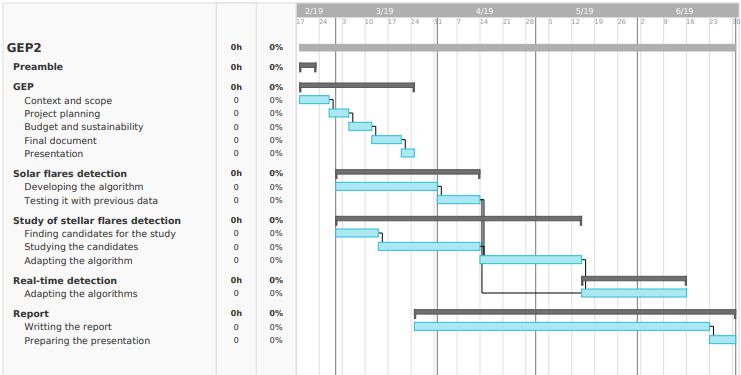
\includegraphics[width=0.9\linewidth]{images/GanttChart.png}
	\caption{Gantt chart with the planning of the project }
\end{figure}
	

%%%%%%%%%%%%%%%%%%%%%%%%%%%%%%%%
%%%%%%%%%% Action plan %%%%%%%%%%
%%%%%%%%%%%%%%%%%%%%%%%%%%%%%%%%

\subsection{Action plan}

Our idea is to work in the presented order as planned in the the previous sections, some tasks depend on previous ones to be finished to continue, and others are going to be done in parallel, like writing the report.

The project was been scheduled as previously presented, but if the dedication for some of the tasks is more than expected, the schedule should be modified as the project progresses to adapt to these situations. Another factor that might have an effect on our scheduling are some problems that might appear during the development of the project, this may cause delays and that will force us to reschedule the project planning, some of which are presented below.

As seen in the methodology section, a weekly meeting with the supervisor is held, so if any delays have appeared during the week, the schedule can be changed accordingly.

\paragraph{Understanding of the problem}

The problem has a considerable physics background that I, as a Computer Science student, lack the knowledge to completely understand it. Although a basic knowledge in the field will suffice for developing the algorithms, not having a background in physics might lead to confusion at some point, and will make it more difficult to understand what does the algorithm have to exactly do.

\paragraph{Understanding previous algorithms}

It is often difficult to understand code that has not been written by oneself, let alone understanding complex algorithms without any previous knowledge. This could be another possible obstacle, as the study of the previously developed algorithms will play an important role in the development of ours.

\paragraph{Bugs}

As we will be writing code it is clearly possible that we face problems with bugs that may appear in the process.

\subsection{Resources}

Several tools that will be studied in detail in the following section, along with the cost they imply, will be needed for the development of the project. These resources can be classified in three major groups:

\paragraph{Software resources}

Many software tools will be needed for the development of the project, although all of them will be free and open-source. All the used tools are listed in the next section, although some of the main ones are Git, which will be used for version control, everything will be running on Linux and \LaTeX\ will be used for the reports. 

\paragraph{Hardware resources}

In this case only a computer will be needed, we will be relying on data that has been obtained using far more complex technologies (all the satellites and hardware involved in GNSS) but a computer and its peripherals will be the only hardware used during the project.

\paragraph{Human resources}

One person will be developing the project and will have three roles: the project manager (time management and writing the report), software developer (developing the necessary algorithms) and tester (testing said algorithms).

%%%%%%%%%%%%%%%%%%%%%%%%%%%%%%
%%%%%%% Cost estimation %%%%%%
%%%%%%%%%%%%%%%%%%%%%%%%%%%%%%

\section{Cost estimation}

In the following sections, an estimation of the cost is presented. These are going to be divided in four major sections: hardware, software, human resources and indirect costs. Because  some of the tasks will use the same resources, they have been grouped, but those that use different resources will be studied in a different section.

\subsection{Software resources}

\paragraph{Common resources}

\begin{table}[h!]
	\centering
	\def\arraystretch{1.2}
	\begin{tabular}{|c c c c c|} 
		\hline
		Product & Units & Price & Useful life (years) & Amortization \\ [0.5ex] 
		\hline\hline
		Ubuntu 18.04 & 1 & 0 \euro & - & 0 \euro \\ 
		\hline
		Google Chrome & 1 & 0 \euro & - & 0 \euro \\
		\hline
		Evince & 1 & 0 \euro & - & 0 \euro \\
		\hline\hline
		Total &  & 0 \euro &  & 0 \euro \\
		\hline
	\end{tabular}
	\caption{Software costs}
\end{table}

\newpage

\paragraph{Developing the algorithms}

\begin{table}[h!]
	\centering
	\def\arraystretch{1.2}
	\begin{tabular}{|c c c c c|} 
		\hline
		Product & Units & Price & Useful life (years) & Amortization \\
		\hline\hline
		Git & 1 & 0 \euro & - & 0 \euro \\ 
		\hline
		GitHub & 1 & 0 \euro & - & 0 \euro \\
		\hline
		Sublime Text 3 & 1 & 0 \euro & - & 0 \euro \\
		\hline
		Python & 1 & 0 \euro & - & 0 \euro \\
		\hline
		GNSS Data & 1 & 0 \euro & - & 0 \euro \\
		\hline
		GFortran & 1 & 0 \euro & - & 0 \euro \\
		\hline\hline
		Total &   & 0 \euro &  & 0 \euro \\
		\hline
	\end{tabular}
	\caption{Software costs}
\end{table}

\paragraph{GEP and writing the report}

\begin{table}[h!]
	\centering
	\def\arraystretch{1.2}
	\begin{tabular}{|c c c c c|} 
		\hline
		Product & Units & Price & Useful life (years) & Amortization \\
		\hline\hline
		LibreOffice & 1 & 0 \euro & - & 0 \euro \\ 
		\hline
		LaTeX & 1 & 0 \euro & - & 0 \euro \\
		\hline
		TeamGantt & 1 & 0 \euro & - & 0 \euro \\
		\hline\hline
		Total &   & 0 \euro &  & 0 \euro \\
		\hline
	\end{tabular}
	\caption{Software costs}
\end{table}

\subsection{Hardware resources}

The following table contains the costs of the hardware that is going to be used for the project. These resources are common to all phases.

\begin{table}[h!]
	\centering
	\def\arraystretch{1.2}
	\begin{tabular}{|c c c c c|} 
		\hline
		Product & Units & Price & Useful life (years) & Amortization \\
		\hline\hline
		Asus X555L & 1 & 750 \euro & 6 & 60 \euro \\ 
		\hline
		PC devices & 1 & 200 \euro & 6 & 20 \euro \\
		\hline\hline
		Total &   & 950 \euro &  & 80 \euro \\
		\hline
	\end{tabular}
	\caption{Hardware costs}
\end{table}

\subsection{Human resources}

The project is going to be developed by one person, which will have to be the project manager, software developer and tester. 

We estimated in the planning section a total dedication time for the project of 550 hours, so here we present an estimation of the distribution of those hours between the roles and the cost of each.

\begin{table}[h!]
	\centering
	\def\arraystretch{1.2}
	\begin{tabular}{|c c c c |} 
		\hline
		Role & \euro/hour & Hours & Cost \\
		\hline\hline
		Project manager & 45 & 100 & 4500 \\
		\hline
		Software developer & 40 & 300 & 12000 \\
		\hline
		Tester & 30 & 150 & 4500 \\
		\hline\hline
		Total &  & 550 & 21000 \\
		\hline
	\end{tabular}
	\caption{Human resources costs}
\end{table}

\subsection{Indirect costs}

Indirect costs of elements that will be needed in order to use the previous hardware are shown in table 6:

We can estimate the energy expenditure during the project assuming the computer consumes an average of 200 watts per hour. If we plan to use it during the 550 hours of the project, we cam estimate a total of 110 kW spent.

\begin{table}[h!]
	\centering
	\def\arraystretch{1.2}
	\begin{tabular}{|c c c c|} 
		\hline
		Product & Use & Price & Estimated cost \\
		\hline\hline
		ADSL & 4 months & 40 \euro/month & 160 \euro\\
		\hline
		Electricity & 110 kWh & 0.1067 \euro/kWh & 11.7 \euro\\
		\hline\hline
		Total &  &  & 172 \euro\\
		\hline
	\end{tabular}
	\caption{Indirect costs}
\end{table}

\subsection{Budget per task}

In the following table we can see an estimation of the total cost of the project distributed among the tasks presented in the planning section, according to the dedication time of each of these tasks and the total cost of the project:

\begin{table}[h!]
	\centering
	\def\arraystretch{1.2}
	\begin{tabular}{|c c|} 
		\hline
		Task & Estimated cost\\
		\hline\hline
		Introduction to the problem & 1106 \euro\\
		\hline
		GEP & 4424 \euro\\
		\hline
		Feasibility of the detection of flares from far-away stars & 4424 \euro\\
		\hline
		Detection of solar flares with no information about the location of the Sun & 4424 \euro\\
		\hline
		Detection of stellar flares in real-time & 3318 \euro\\
		\hline
		Writing the report and final presentation & 4424 \euro\\
		\hline\hline
		Total & 22122 \euro\\
		\hline
	\end{tabular}
	\caption{Budget per task}
\end{table}

\newpage

\subsection{Total budget}

In the following table, the total cost of the project can be seen, estimated using data seen in the previous tables.

As we can see, there is no software cost because only open-source or free tools have been used.

\begin{table}[h!]
	\centering
	\def\arraystretch{1.2}
	\begin{tabular}{|c c|} 
		\hline
		Resource & Estimated cost\\
		\hline\hline
		Software & 0 \euro\\
		\hline
		Hardware & 950 \euro\\
		\hline
		Human resources & 21000 \euro\\
		\hline
		Indirect costs & 172 \euro\\
		\hline\hline
		Total & 22122 \euro\\
		\hline
	\end{tabular}
	\caption{Total cost of the project}
\end{table}

\subsection{Budget control}

As seen in the planning section, some of the tasks may take longer than estimated because of unexpected difficulties, which would in turn increase the total cost of the project. So we have to consider the fact that these delays could lead to an increase in the total cost of the project. 

Weekly meetings are held to check that everything is going as scheduled, so if any problem appears we can try to reschedule the planning of the project and avoid as much extra costs as possible.

Although unlikely, hardware faults might occur that would require more resources, but the main factor that might influence the budget during the project is time, which would increase the amount of work hours done by either the project manager, the software developer or the tester.

\section{Sustainability}

The form presented by EDINSOST has helped me reflect on how, although in some courses during the degree the relation between Computer Science (or engineering in general) and sustainability has been studied, as engineers, we don't usually consider these factors on our own, such as the environmental or social impact. The economical impact is something usually considered, specially by project managers, but seldom is the effect of the technology on the environment taken into consideration.

I have realized how in many of the projects I collaborate, I do not usually stop to think about the impact they are having, for example, on the environment, and how I have no experience in these fields, specially in the economic management part. Therefore, I hope I can gain some experience by studying these aspects more in depth and the impact of the project in them. \\

In this section we will focus on evaluating the impact of our project by studying its sustainability in three different aspects: environmental, economical and social.

The analysis is going to be based on the application of the following sustainability matrix which is scored in a [0,10] range and then will study each of the three main aspects:

\begin{table}[h!]
\begin{center}
	\def\arraystretch{2.2}
	\begin{tabular}{|c|c|c|c|}
		\hline
		\thead{} & \thead{\textbf{PPP}} & \thead{\textbf{Exploitation}} & \thead{\textbf{Risks}} \\
		\hline
		\textbf{Environmental} & \makecell{(2) Design \\ consumption} & \makecell{(2) Ecological\\ footprint} & \makecell{(2) Environmental\\ risks}\\
		\hline
		\textbf{Economic} & \makecell{(4) Resources needed} & (2) Cost & \makecell{(7) Human resources}\\
		\hline
		\textbf{Social} & \makecell{(9) High personal \\ impact} & \makecell{(5) Medium social\\ impact} & \makecell{(2) Low social risks}\\
		\hline
	\end{tabular}
\caption{Sustainability matrix}
\end{center}
\end{table}

\subsection{Environmental sustainability}

During the project we are going to use the minimum amount of resources possible, which have been presented in the Cost estimation section. Because what we are going to use is mainly software, the resource from the project which will have an environmental impact is going to be the energy spent by the devices running during the project (the computer).

Furthermore, if the project is successful, it would present an alternative to currently working satellites that detect Gamma-Ray Bursts (GRB), like the Gamma-ray Large Area Space Telescope (GLAST) or weather satellites like the Geostationary Operational Environmental Satellite (GOES).

As seen in its specification manual (https://www.nasa.gov/pdf/221503main\_GLAST-041508.pdf) GLAST needs about 1500 watts average over an orbit, which is significantly more than the consumption of the computer that we have estimated before: 110 kWh. The telescope, however, is equipped with solar panels that can supply up to 3122 watts in sunlight. 

While our alternative would not obtain results with the precision and information that these missions aim to achieve, some results would be similar, so we can also consider the difference in environmental impact between both.

The larger environmental impact of the GLAST mission, however, lies in the design, build and launch of the telescope. While information about the cost of the previous factors is available and will be studied in the next section, there is no information provided regarding its environmental impact, although we can say that it likely has a considerably larger one than that of our project, in which only a computer is used.

In conclusion, the project’s resources are mainly software and the factor with the biggest environmental impact will be the energy expenditure of the computer, which is significantly lower than that of the currently existing alternatives.

\subsection{Economic sustainability}

In previous sections we have studied the cost of our project (hardware, software and human resources). From an economical point of view, our project presents an alternative to telescopes like GLAST or GOES. Albeit less precise and equipped, some of its aspects and purposes are shared.

The  cost to design, build and launch GLAST, for example, had a total international contribution of 690 US dollars. Considering our project relies only on free or open-source data and software, it would be offering an alternative with a lower economical impact. 

It would be difficult to do this project with a lower cost, considering the only resource that has an economical impact besides the human work is the hardware (a computer). It would be difficult to lower the costs of this area considering a computer is needed for most computer science projects.

\subsection{Social sustainability}

Personally, the project is very relevant to me. I wanted to work on a project to see how computer science could be applied to a field like astronomy or physics. I think the project and algorithms we are developing are a good example of the place CS has in this fields and the role it plays.

It has also helped me gaining experience in terms of information retrieval and research. Both writing reports like this one, planning projects and researching information from reputable sources that can be used in our project.

If the project is successful, it could turn into a useful tool for astronomers that could be used as an astronomical instrument to measure the Sun’s EUV using only open-source GPS data, rather than a dedicated telescope, which would be a useful, less expensive alternative.

\chapter{Background}
As the project has a large background in physics and astronomy, some of the relevant topics that are going to be studied are introduced: Global Navigation Satellite Systems, the Ionosphere, Stellar Flares and Gamma-Ray Bursts.

\section{Global Navigation Satellite Systems}

\paragraph{GNSS and GPS}

These two terms may lead to confusion as Global Navigation Satellite Systems (GNSS) is the generic term for all satellite navigation systems. The Global Positioning System (GPS), in particular, is the United States' GNSS system, the world's most used GNSS. Other systems, for example, are the European Galileo or Russian GLONASS \cite{hegarty2008evolution}.

Global Navigation Satellite Systems use satellites to determine the position of a given object or device in terms of latitude, longitude and height. 

\paragraph{Positioning}

In short, GNSS works as follows: out of all the GNSS satellites orbiting Earth, at least four of them are constantly visible from a specific point and transmitting information at a certain frequency. When a device receives a signal from one of them, the distance to the satellite can be calculated by means of the time required to reach it and the speed of light. As many variables might affect the speed of light such as the medium through which it is propagating, this estimation of the distance is called \textbf{pseudo-range}. 

Thus, the location of the receiver can be estimated using a technique called \textbf{trilateration}. Having three spheres around each of the satellites with the pseudo-range as their radius, the intersection of these spheres yields the location of the receiver \cite{hofmann2007gnss}. 

\paragraph{Ionospheric Pierce Points}

Ionospheric Pierce Points (IPP) are going to be very relevant throughout the development of the project. These will be the locations that we are going to use for our measurements, not those of satellites or receivers. A Ionospheric Pierce Point is the point where the line between the satellite and a receiver intersect with the ionosphere, where the Total Electron Content can be estimated. \cite{fu2000satellite}

\paragraph{The International GNSS Service}

In 1998 the International GNSS Service (IGS) was created as a collaboration of several members of the scientific community: Center for Orbit Determination in Europe (CODE), (European Space Agency) ESA, Jet Propulsion Laboratory (JPL) and Polytechnic University of Catalonia (UPC). This voluntary federation has made available open access GNSS data since its creation \cite{igswebsite} \cite{dow2009international}. 

Its data is provided by more than 300 GPS receivers around the globe and is processed by the previous institutions which compute the global distribution of the Total Electron Content (TEC) \cite{hernandez2009igs}.

GNSS is a key component to this project because, as mentioned before, many variables can affect the speed of light and therefore the time it takes for the transmitter's signal to be intercepted by the receiver. One of these variables is the electron content of the layer of the atmosphere where GNSS satellites operate: the ionosphere.

\section{Ionosphere}

The ionosphere is a layer of the Earth’s atmosphere that lies 75-1000km above the surface of the planet \cite{ionospherestandford}. 

High energy from Extreme UltraViolet (EUV) and X-ray radiation can cause its atoms to be ionized and create a layer of electrons \cite{noaa2ionosphere}. Due to these free electrons and ionized molecules, it is capable of affecting radio wave propagation, thus having an effect on Global Navigation Satellite Systems (GNSS) technology, this phenomena allows these satellites to be used as a global scanner for the ionosphere \cite{hernandez2011ionosphere}. 

The main physical quantity used for describing the electron content of the ionosphere is the \textbf{Total Electron Content (TEC)}, the TEC is the total number of electrons between two points $(r1,r2)$ along a cylinder of base $1m^2$. 
Slant TEC (STEC), in particular, can be defined as the TEC in which $r1$ and $r2$ are a satellite and a receiver’s positions \cite{singh2015gps}. 

The unique properties of the ionosphere enable us to use the data provided by the GNSS technology to study stellar flares, a powerful phenomena that occurs in many stars across the universe.

\section{Stellar flares}

Flares from stars, in particular those that have the Sun as a source (more noticeable due to its proximity) are sudden flashes of brightness in the surface of stars which release large amounts of energy across the whole electromagnetic spectrum\footnote{X-rays and Extreme Ultraviolet (EUV) radiation}.
Flares that have the Sun as a source can increase the electron content of the ionosphere and have an effect on waves passing through it, affecting satellite communications and causing a delay. This phenomena is the key element of the project, as it enables us to study these events.

Satellites can also be harmed by this effects: the flares heat up the outer atmosphere, which in turn increases the drag on these satellites reducing their lifetime in orbit \cite{hernandez2012gnss}.

The previous phenomena applies to flares originating from the Sun, whether a flare that has a star from outside the Solar System as a source has an effect on the Earth’s atmosphere or not is one of the topics that is going to be studied in this project, as the distance may reduce their effect on the Earth.

\section{Gamma-Ray Bursts}

Throughout the project, in particular when studying the feasibility of stellar flares detection, another type of event will be mentioned and studied as well: Gamma-Ray Bursts (GRBs):

GRBs are highly energetic explosions that occur in distant galaxies, releasing large amounts of radiation, in particular Gamma rays, hence the name of the event. These bursts, despite being millions of light years away from Earth are so powerful they might still have an impact on the ionosphere, like the aforementioned stellar flares. 
The main difference with flares originating from stars is that GRBs are thought to be originated from the death of massive stars, that is, supernovas.

Despite not being a stellar flare, the phenomena we aim to detect, this event is going to be studied in the following section to test the currently working algorithms, mainly for two reasons: it has been studied and cataloged by telescopes such as the Fermi Observatory and there’s is available information that we can use for our study, and the large amounts of energy they emit it could mean GRBs are a more feasible target to detect.
\chapter{Study on the feasibility of stellar flare detection}

Flares from far-away stars and Gamma-ray Bursts, albeit more powerful than flares that have the Sun as their source, may not be possible to detect due to the large distances that separate them from our measurement tool: the ionosphere.

Before starting to adapt the algorithm for detecting solar flares to this scenario, a study was conducted parallel to its development, to see if the energy from flares originating in far-away stars could be detected using the already existing method, namely the GNSS Solar Flare Activity Indicator (GSFLAI) algorithms \cite{hernandez2012gnss}.

To study if this was feasible, the algorithms were run on certain candidates of flares and GRBs to see if they could be detected.

The project supervisor, Manuel Hernández-Pajares, who as mentioned before has previously performed several studies on the subject, provided the GSFLAI algorithm to test the candidates. The GSFLAI algorithm takes into consideration the location of the source (the Sun) to see if there's a relation between an increase in the VTEC of the ionosphere and the solar-zenith angle to determine if this increase is caused by a solar flare. [GNSS measurement of EUV photons flux rate
during strong and mid solar flares]

However, its execution may take up to 2 hours, because of this the aim was to:

\begin{itemize}
	\item Find a database for possible candidates, several online archives with information about previously recorded Gamma Ray Bursts were considered.
	\item Select an appropriate source of this pool of candidates by writing a quick script that yielded an ordered list of the best candidates based on certain factors, instead of selecting a random source.
\end{itemize}

\section{Sources of data and possible candidates}

The three main databases we considered for the study were:

\begin{itemize}
\item The GRB collection website of Jochen Greiner, scientist at the Max-Planck-Institute for extraterrestrial Physics (MPE) \cite{greinergrb},  which offers a collection of detected GRBs by different telescopes and observatories.
\item The Magnetar Outburst Online Catalog (MOOC), developed by the Institute of Space Sciences (CSIC-IEEC, Barcelona) \cite{moocgrbs}. We also had the pleasure to meet one of the leaders of this project, Nanda Rea, and discuss
\item The Neil Gehrels Swift Observatory website and archive by the National Aeronautics and Space Administration (NASA), Goddard Space Flight Center \cite{swiftnasa} which contains an archive of detected GRBs by the Swift observatory and is constantly updated.
\end{itemize}

Because of the layout of the website and how the data could be accessed, the option with which we started was the Swift Database, as the data could be visualized in an HTML table and was easily accessible.

\section{The Neil Gehrels Swift Observatory and its data}

The Swift Observatory is a NASA mission with international participation, designed to observe GRBs and their afterglows to study topics such as the origins of GRBs or what they can reveal about the early stages of the universe \cite{roming2005swift}. The observatory is equipped with three main instruments that work with each other to study GRBs \cite{gehrels2004swift} \cite{swiftnasa}:

\begin{itemize}
\item The \textbf{Burst Alert Telescope (BAT)}, tasked with detecting the GRBs and computing their positions. This triggers the spacecraft to point the other telescopes to the burst so it can be studied in more detail. 
\item The \textbf{X-ray Telescope (XRT)}, used for studying the X-ray radiation and taking images of the bursts which in turn help increase the accuracy of the location estimation.
\item The \textbf{UV/Optical Telescope (UVOT)}, which serves a similar purpose to the XRT, but studies the ultraviolet band of the spectrum. 
\end{itemize}

For each detected GRB, the data obtained by the different telescopes is given. The parameters that are relevant to our study and determine the fitness of each of the candidates are:

\begin{itemize}
\item The \textbf{name of the burst}, given by the date it was detected. For example, the GRB named 190220A was detected the 20th of February of 2019.
\item The \textbf{Universal Time (UT)} of the detection, that is, hh:mm:ss of the day given by the name.
\item The fluence detected by the BAT component, in units of keV. that is.
\item The \textbf{UVOT magnitude}, measured by the UV Telescope.
\item The location that triggered the detection, given as  \textbf{Right Ascension (Ra)} and \textbf{Declination (Dec)}.
\end{itemize}

Right Ascension and Declination are two concepts similar to longitude and latitude, respectively, used to describe the location of objects in the sky, in particular in a sphere of infinite radius that with the Earth as its center called the \textbf{celestial sphere}.

Taking this into account, Right Ascension is the equivalent of longitude, expressed in degrees (or more commonly in hours, minutes and seconds) and Declination, the equivalent of latitude, is expressed in degrees between the two poles: +90º and -90º. \cite{nasareferencesystem}

This reference system is used to describe the position of objects in the sky, and it is the one used by the Swift telescope to specify the location of the sources. Afterwards these concepts will play an important role when computing the angle formed between the source and the Sun.

\section{Objective function}

Our main goal in this section was to obtain a list of GRB candidates ordered from more to less probable to be detected by the algorithm, that is, their fitness. To obtain this score we had to define an objective function, taking into consideration two factors:

\begin{itemize}

\item The \textbf{strength} of the burst, given by the UVOT magnitude. If this value was not available (as it was the case with many of the candidates) the BAT fluence was considered as its strength. This values were already given by the archive and no additional computations were required.

\item The \textbf{angle between the burst and the Sun}, this was an important factor because bursts having an effect on the night hemisphere should be more noticeable than those hitting the day one, where the Sun has a bigger influence.

\end{itemize}

\paragraph{Computing the angle}

As mentioned before, the Swift archive gives us the Right Ascension (Ra) and Declination (Dec) where the source is thought to be located.

The location of the Sun, on the other hand, is unknown. But we do know the time when the burst was detected.

The supervisor, Manuel Hernández-Pajares, provided me an algorithm which takes date (year, month, day and UT) and a planet of the Solar System (or the Sun, our case) as the input and returns its location in the celestial sphere, that is, its Ra and Dec. 

This algorithm belongs to the \textbf{Starlink Project} (Rutherford Appleton Laboratory), which provided open-source software like the one at hand to astronomical institutions. Although it was shut down in 2005, the code still remains and we could use it for our study \cite{starlinkproject}.

Knowing the location of the GRB: ($\delta_{g}, \alpha_{g}$), declination and right ascension, respectively. And that of the Sun: ($\delta_{s}, \alpha_{s}$), the cosine of the angle between both can be computed and used as a parameter for the objective function.

This computation is done by performing the dot product of the two unit vectors that can be obtained from the Ra and Dec of the objects given by the following formulas: \cite{de donde salen las formulas}  TODO: arreglar esta cita

\begin{equation} \label{eq:1}
	unitVectorGRB =	
	\begin{bmatrix}
	\cos\delta_{g} * \cos\alpha_{g} \\ 
	\cos\delta_{g} * \sin\alpha_{g} \\
	\sin\delta_{g}
	\end{bmatrix}
\end{equation}

\begin{equation} \label{eq:2}
	unitVectorSun =	
	\begin{bmatrix}
	\cos\delta_{s} * \cos\alpha_{s} \\ 
	\cos\delta_{s} * \sin\alpha_{s} \\
	\sin\delta_{s}
	\end{bmatrix}
\end{equation}

\begin{equation} \label{eq:3}
	\cos angleSunGRB = unitVectorGRB \cdot unitVectorSun
\end{equation}\\

The code for the previous computation is shown here:\\

\begin{lstlisting}[language=Python, caption=Python function for computing the angle]
def scorePosition(sunRa, sunDec, ra, dec):
	# If Ra and/or Dec are n/a, return 0, else, compute the dotProduct
	if ra == 0 or dec == 0:
		return 0
	
	coordSun = [math.cos(sunDec)*math.cos(sunRa),
	math.cos(sunDec)*math.sin(sunRa), 
	math.sin(sunDec)]
	
	coordGRB = [math.cos(dec)*math.cos(ra),
	 math.cos(dec)*math.sin(ra),
	  math.sin(dec)]
	
	angle = math.acos(coordSun[0]*coordGRB[0] +
	coordSun[1]*coordGRB[1] +
	coordSun[2]*coordGRB[2])
	
	angle = angle*180/math.pi
	
	return angle
\end{lstlisting} 





\section{Obtaining the data}

Regarding the scrapping of the website to parse the data and obtain this ordered list, \textbf{Python} was chosen because the problem required a quick implementation, and Python’s libraries offered a great tool to develop a simple solution as quick as possible.

In the script, the website with the table of bursts (see figure x) is scrapped using Python’s \textbf{BeautifulSoup} library, which has an HTML and XML parser that allows us to easily select and obtain data from a given website.

Insertion sort was used so we could insert every considered GRB into a list of sorted candidates as we were traversing the table. 



Regarding the distribution of weight between both factors, strength and angle, we ….

The best 10 candidates of the resulting sorted table (pie de pagina: bursts registered up to the 26th of February of 2019), is shown here:

We proceeded to study these bursts

\section{Results}

\chapter{Solar flare detection}

\textbf{COMPLETO Y REVISADO}

Before developing the main solar flare detection algorithm a first study is presented that targeted a powerful solar flare for which we knew the time of the event and therefore, the location of the Sun.

Although the aim of the main algorithm is detecting the solar flare without taking into consideration the position of the Sun, this study was done to understand how the core of the algorithm works: studying the correlation between the cosine of the solar-zenith angle and the VTEC content.

This chapter also provides an introduction to the formatting and use of the Global Navigation Satellite Systems data (GPS in this case) and how the main parameters necessary for the algorithms are computed.

\section{Data}

\subsection{GPS Data}

As we have seen in previous sections, the International GNSS Service (IGS) has made available open access GNSS data since its creation. The Crustal Dynamics Data Information System (CDDIS) is a central data archive for the NASA's Crustal Dynamics Project (CDP), dedicated to archiving space geodesy data for research. This archive has been storing and providing access to the GNSS data generated by the IGS since 1992.

Figure \ref{fig:exampleCDDIS} (a) shows how data is stored in de CDDIS server (\url{ftp://cddis.nasa.gov/gps/data/hourly/}).

The files in this server contain raw GPS data that is then pre-processed to obtain VTEC maps in the form of \textbf{ti} files. An example diagram of this complex, several step procedure is shown in figure \ref{fig:exampleCDDIS}(b), extracted from the paper \textit{"The IGS VTEC maps: a reliable source of ionospheric information since 1998"} \cite{hernandez2009igs} by Manuel Hernández-Pajares, which offers a detailed explanation of this process. 

\begin{figure}[!htb]
	\begin{subfigure}[b]{0.3\textwidth}
		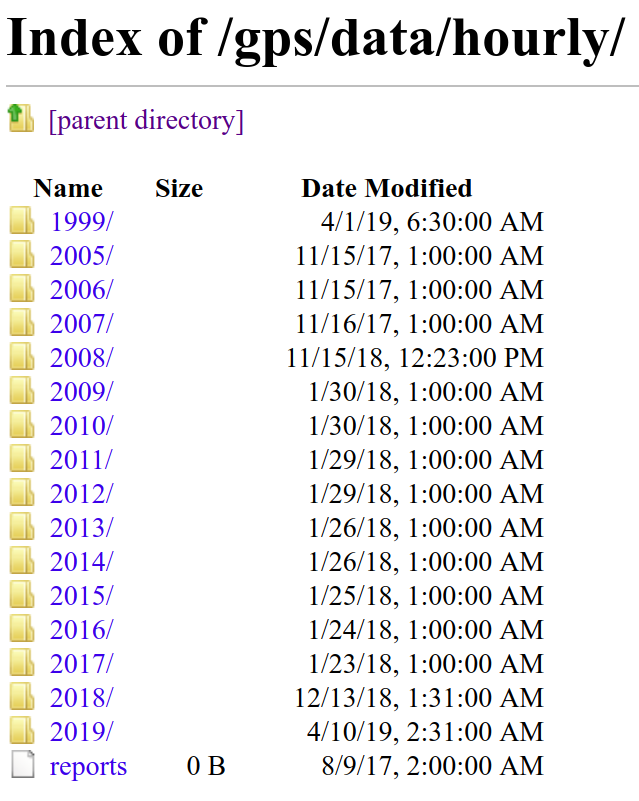
\includegraphics[width=\linewidth]{images/ch4/FTPNASA.png}
		\caption{Files}
	\end{subfigure}
	\hfill
	\begin{subfigure}[b]{0.5\textwidth}
		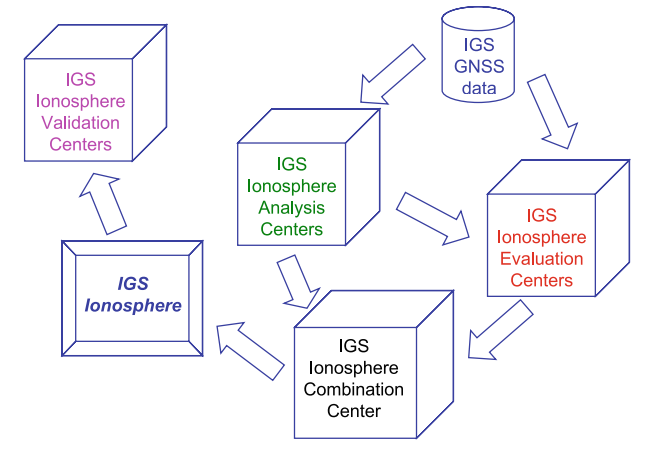
\includegraphics[width=\linewidth]{images/ch4/DataFlowIGS.png}
		\caption{Data flow}
	\end{subfigure}
	\caption{CDDIS server (a) and data flow to obtain IGS data (b)}
	\label{fig:exampleCDDIS}
\end{figure}

However, for this and the following section, only the pre-processed ti files of past dates were needed, as detecting the flares in real time is a task that will be discussed later in the project, in which this pre-processing will have to be taken into consideration. The project supervisor, Manuel Hernández-Pajares, provided me with some of data sets to use as input for the algorithms, along with information about the formatting of this files.

\subsection{Formatting}

The ti files contain several rows of pre-processed GPS data. Each row has a Receiver Id. and a Transmitter Id., therefore, for each row we have the Ionospheric Pierce Point between the Receiver and Transmitter. Each IPP has several parameters that are relevant for our computations:

\begin{itemize}
\item The \textbf{GPS time}
\item The \textbf{Receiver Id.}
\item The \textbf{Transmitter Id.}
\item The \textbf{double derivate of Li}
\item The \textbf{xmappingion}
\item The \textbf{right ascension} and \textbf{declination} of the IPP
\end{itemize}

\begin{minipage}{\linewidth}
\begin{lstlisting}[caption=Format of the ti file]
Field number | Example value | Description
[...]
3 		0.008333333333		GPS time/hours (tsecdayobs/3600.d0)
4 		cand							Receiver Id.
5 		3									Transmitter Id.
[...]
21 		-0.5131586E-02		d2li
[...]
43 		0.1565765332E+01		xmapping_ion
44 		334.449							xraion
45 		33.092							xlation
[...]
\end{lstlisting}
\end{minipage}
The files also contain the right ascension and declination of the \textbf{Sun}, which will be used in the last chapters to study the error of the algorithm's estimations.

\subsection{The Halloween Solar Storm: X17.2 flare}

The data set we used was that of the so-called Halloween Storm, a powerful solar storm that took place from October to early November in the year 2003. In particular, we will try to replicate the results shown in figure \ref{fig:halloweenPaper}, shown in the paper \textit{"GNSS measurement of EUV photons flux rate during strong and mid solar flares"} for a poweful flare that took place in October 28th, 2003 \cite{hernandez2012gnss}.

\begin{figure}[!htb]
	\begin{centering}
		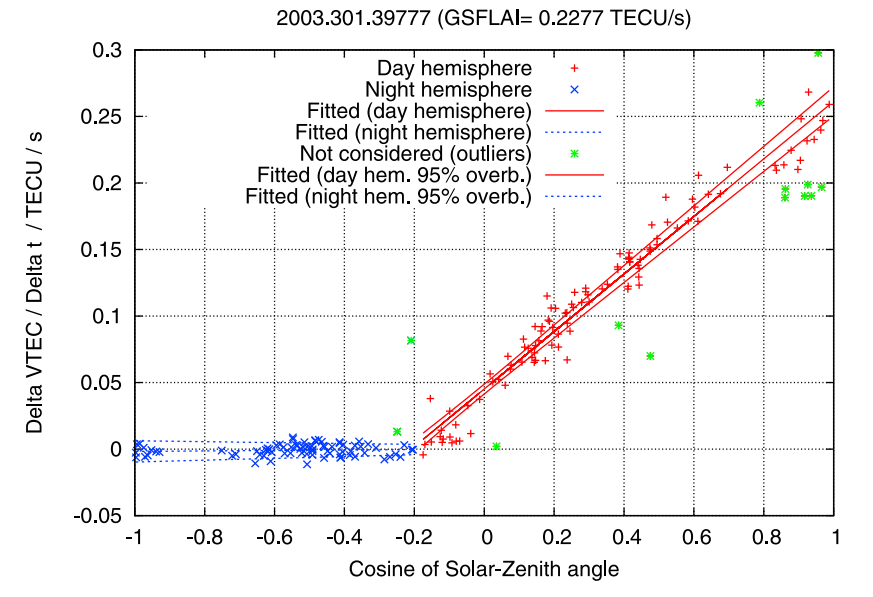
\includegraphics[width=0.5\linewidth]{images/ch4/halloweenPaper.png}
		\caption{VTEC as a function of the cosine of the solar-zenith angle}
		\label{fig:halloweenPaper}
	\end{centering}
\end{figure}

As we can see the plot of the flare called X17.2 took place exactly at 2003.301.39777 (year.day.seconds of GPS time). In hours, 39777 seconds of a day is $39777s * 1h/3600s = 11.049...h$, around 11AM. 

The ti files provided contained data from 10.5h to 11.5h (with a sampling rate of 30 seconds), so that we could see the VTEC distribution throughout the day.

With this data we can compute the two parameters that will yield the plot shown in figure \ref{fig:halloweenPaper}: the \textbf{VTEC value} and the \textbf{cosine of the solar-zenith angle}.

\section{Vertical Total Electron Content (VTEC)}

Fisrt we wanted to obtain VTEC distribution throughout the day, to visually see if any spikes appeared confirming that the moment we were going to study based on the paper was correct.

For each epoch in our data set (from 10.5 to 11.5 with a sampling rate of 30 seconds) we needed to compute an estimation of the VTEC value.

\subsection{Computing the VTEC}

As we have mentioned before, one of the main paramenters relevant to the computation is the \textbf{double derivate of LI}, the d2li field in the ti file. The Li is the "ionospheric combination of carrier phases" \cite{hernandez2012gnss}, a direct measurement of TEC. Because this is a derivative, it is the \textbf{increment in VTEC}, this will be observed in figure \ref{fig:vtecDistribution}.

The VTEC increment can be estimated using the following operation:

\begin{equation} \label{eq:1}
	\frac{d^{2}V}{dt^{2}} = \frac{d^{2}Li}{M}
\end{equation}

Where $M=\frac{1}{\cos Z}$ is the "ionospheric mapping function", the inverse of the cosine of the satellite-zenith angle that we have for each IPP. \cite{hernandez2012gnss}. This is the \textbf{xmappingion} field in the ti file.

Therefore, we can estimate the VTEC increment of an IPP by dividing the two given parameters:
\begin{equation} \label{eq:2}
	\Delta V \approx \frac{d^{2}Li}{M}
\end{equation}

Although the data that will be used throughout the project is going to be $\Delta V$, the VTEC increment, it will be referenced as simply VTEC from now on for readability.

\paragraph{Implementation}

Below is the code used to compute the VTEC value in Fortran that we will use to replicate the plot from figure \ref{fig:halloweenPaper}.

\begin{minipage}{\linewidth}
\begin{lstlisting}[language=Fortran, caption=Simple Fortran function to compute the VTEC value]
double precision function estimateVTEC (mapIon, d2Li)
	implicit none
	double precision, intent(in) :: mapIon, d2Li
	double precision :: vtec
	
	vtec = d2Li/mapIon
	return
end function estimateVTEC
\end{lstlisting}
\end{minipage}

\subsection{Distribution throughout the day}

Because the only operation that had to be performed was the previous division, for plotting the distribution throughout the day a simple AWK script was used to filter out the two necessary fields from the data file and print the resulting value as a function of time. 

\begin{minipage}{\linewidth}
\begin{lstlisting}[language=Awk, caption=AWK script to estimate the VTEC]
{
	/a/
	d2li = $21;
	mappingFunc = $43;
	vtec = d2li/mappingFunc;
	print $3 " " vtec
}
\end{lstlisting}
\end{minipage}

\begin{minipage}{\linewidth}
\begin{lstlisting}[language=Bash, caption=Bash script to execute the procedures]
#!/bin/bash
tiDataFile="../data/ti.2003.301.10h30m-11h30m.gz"

zcat "$tiDataFile" | gawk -f previewVTECDistribution.awk > vtecValues
gnuplot -e "set terminal png; set output 'vtecDistribution.png'; set title 'VTEC Distribution'; set xlabel 'Time of the day (hours)'; set ylabel 'VTEC'; set grid; plot \"vtecValues\" using 1:2 with point"
rm vtecValues
\end{lstlisting}
\end{minipage}
\clearpage

The bash script executes the AWK process with the data as the input and outputs n rows with two columns: the \textbf{time of the day} and the \textbf{calculated VTEC}, and finally plots the results using Gnuplot. 

This results can be seen in figure \ref{fig:vtecDistribution}(a), where we can see how the VTEC value evolves throught the day. Visually, a spike can be seen between 11 and 11.2 hours. 

As mentioned before this value is estimated using the derivative of li, because this is the increment in VTEC, we can see that the value becomes negative after the spike, due to the VTEC value decreasing (there is a negative gain ($\Delta V < 0$)).

\begin{figure}[!htb]
	\begin{subfigure}[b]{0.5\textwidth}
		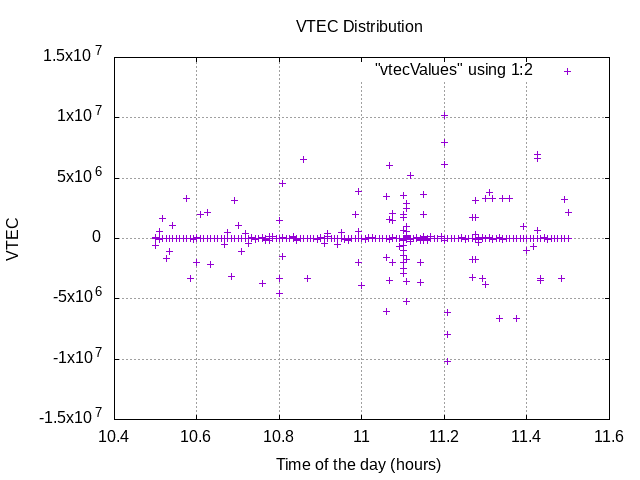
\includegraphics[width=\linewidth]{images/ch4/vtecDistributionGeneral.png}
		\caption{All IPPs}
	\end{subfigure}
	\hfill
	\begin{subfigure}[b]{0.5\textwidth}
		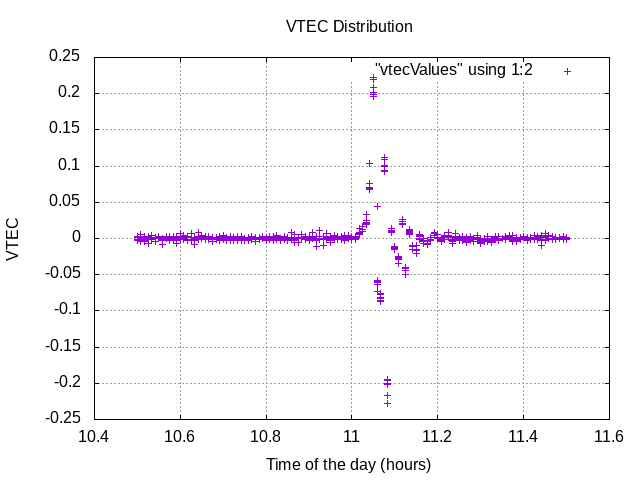
\includegraphics[width=\linewidth]{images/ch4/vtecDistributionVill.png}
		\caption{Villafranca station}
	\end{subfigure}
	\caption{VTEC distribution throughout the day for all IPPS (a) and for IPPs that have Vill as the receiver (b)}
	\label{fig:vtecDistribution}
\end{figure}

To see the event more clearly, though, we can focus on one specific receiver (which will still yield multiple IPPs, as the receiver works with different satellites). For the particular case of the Villafranca, Spain station (identified as Vill in the ti files), we obtain the plot from figure \ref{fig:vtecDistribution}(b). At this time of the day around 11:00h the Sun would have a greater effect on the IPPs of this station due to its location, so the spike can be seen more clearly. 

As mentioned before, the flare took place at 11.05, so we could proceed using the studied data range and this epoch in particular.

\section{Solar-zenith angle}

The solar-zenith angle (denoted $\chi$ from now onward) plays a major role when studying this event: it is the angle formed by the Sun and the Earth's zenith and indicates the effect the flare is having on a particular IPP. It is expected that this variable presents a correlation with the increase in VTEC, which is what we aim to observe in this chapter.

Figure \ref{fig:solar-zenith-angle}, at the end of the chapter, provides a visual representation of this variable that along with the results depicts how it can affect the VTEC value. 

Obtaining the angle between two celestial objects has been shown in the previous section by means of equations \ref{eq:3}, \ref{eq:4} and \ref{eq:5}, when calculating the angle between the Sun and a detected GRB.

\begin{equation} \label{eq:3}
unitVectorObjectA =	
\begin{bmatrix}
\cos\delta_{g} * \cos\alpha_{g} \\ 
\cos\delta_{g} * \sin\alpha_{g} \\
\sin\delta_{g}
\end{bmatrix}
\end{equation}

\begin{equation} \label{eq:4}
unitVectorObjectB =	
\begin{bmatrix}
\cos\delta_{s} * \cos\alpha_{s} \\ 
\cos\delta_{s} * \sin\alpha_{s} \\
\sin\delta_{s}
\end{bmatrix}
\end{equation}

\begin{equation} \label{eq:5}
\cos \beta = unitVectorObjectA \cdot unitVectorObjectB
\end{equation}\\

For this case, though, the cosine of the solar-zenith angle $\chi$ is computed using the IPP's Right Ascension and Latitude (equivalent to declination). The previous dot product can be simplified to:

\begin{equation} \label{eq:6}
\cos \chi = \sin\delta_{IPP}*\sin\delta_{Sun} + \cos\delta_{IPP}*\cos\delta_{Sun}*\cos(\alpha_{IPP} - \alpha_{Sun})
\end{equation}\\

The following Fortran code is the function that implements equation \ref{eq:6} and returns $\cos \chi$:

\begin{lstlisting}[language=Fortran, caption=Computation of the solar-zenith a angle's cosine]
double precision function computeAngle (raIPP, decIPP, raSun, decSun)
	implicit none
	double precision, intent(in) :: raIPP, decIPP, raSun, decSun
	double precision :: solarZenithAngle
	
	solarZenithAngle = sin(decIPP)*sin(decSun) + cos(decIPP)*cos(decSun)*cos(raIPP - raSun)
	return
end function computeAngle
\end{lstlisting}

\section{Results}

Taking $212.338^{\circ}$ and $-13.060^{\circ}$ as the Sun's right ascension and declination, respectively, and the measurements of all IPPs at 11.05 hours, figure \ref{fig:results} shows the plot of the output of our program.

\begin{figure}[!htb]
\begin{centering}
	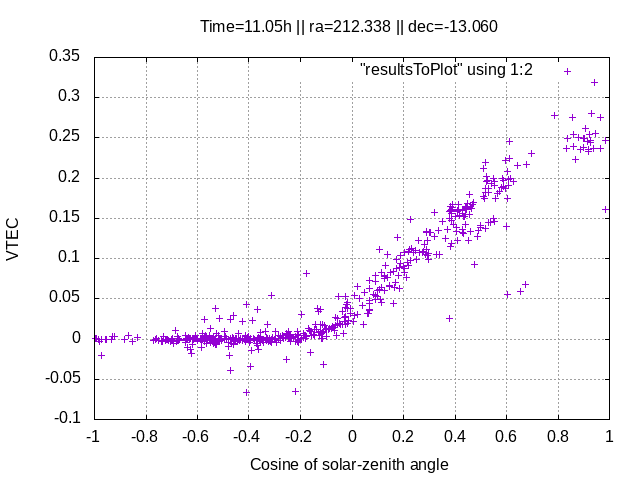
\includegraphics[width=0.5\linewidth]{images/ch4/resultSunTest.png}
	\caption{VTEC value as a function of the solar-zenith angle cosine}
	\label{fig:results}
\end{centering}
\end{figure}

As we can observe, the resulting plot, similar to the one from figure \ref{fig:halloweenPaper}, shows a strong corelation between the cosine of the solar-zenith angle and the VTEC content, which increases from $\cos\chi = 0$ (90$^{\circ}$) to $\cos\chi = 1$ (0$^{\circ}$) (the effect of the Sun on the IPP increases) and it doesn't seem to be affected from $\cos\chi = -1$ (180$^{\circ}$) to $\cos\chi = 1$ (0$^{\circ}$) (when the IPP is in the night hemisphere).

In conclusion, we can see that there appears to be correlation between the two variables. This correlation will be studied in more detail in the following section, where a first approach of the algorithm will be presented to detect the flare without knowing the location of its source.














\chapter{Brute Force Approach}

\textbf{falta acabar seccion mean vtec}

In the previous chapter the correlation between the solar-zenith angle's cosine and the estimated VTEC value was studied. Here, we aim to provide a first, brute force approach, of the \textit{Blind GNSS Search of Extraterrestrial EUV Sources (BGSEES)} algorithm to estimate the location of a EUV source. This approach is done as a first approximation to the problem to see more clearly how the algorithm will work, regardless of its performance.

For this first approach the Sun is used as the source (to check the corectness of the solution). It considers possible Sun locations (with a certain degree of precision) and checks the fitness of each to consider which could be the real location.

\section{Key elements}

\subsection{Mean VTEC as a reliable indicator of the moment of the flare} -> TODO

The first part of the algorithm was, without going into the actual computations regarding the position of the IPPs, the possible Sun locations, etc, finding out when to perform the study, that is, detecting a spike in the VTEC content throughout the provided data range. 
In the previous chapter we already knew the specific moment of the flare: 11.05h, and could work based on this information, but the first step of the algorithm has to determine which moment is going to be studied.

For each epoch\footnote{In our data set the epochs ranged from 10.5 to 11.5, that is, 10:30AM to 11:30AM with a sampling rate of 1/120 hours or 30 seconds} we computed the mean VTEC of all IPPs and returned the epoch which had the highest VTEC mean.

??????An alternative which performs an insertion sort (by inserting the epoch candidates into a priority queue) was also considered and implemented, but for this chapter we only used the epoch with the largest mean.

To see if the mean VTEC could be used as a reliable indicator, the algorithm was tested with all available epochs of the data set, in order to study the effect of this indicator in the resulting estimation of the source's location.

To do this we ordered the different epochs available in our data set by their mean VTEC, inserting them into a priority queue. \\

Figure \ref{fig:differentEpochs} shows the evolution of the correlation coefficient of the best estimated location (a) and its total error (right ascension error + declination error) (b) as the mean VTEC of the epoch decreases.

\clearpage

\begin{figure}[!htb]
	\begin{subfigure}[b]{0.5\textwidth}
		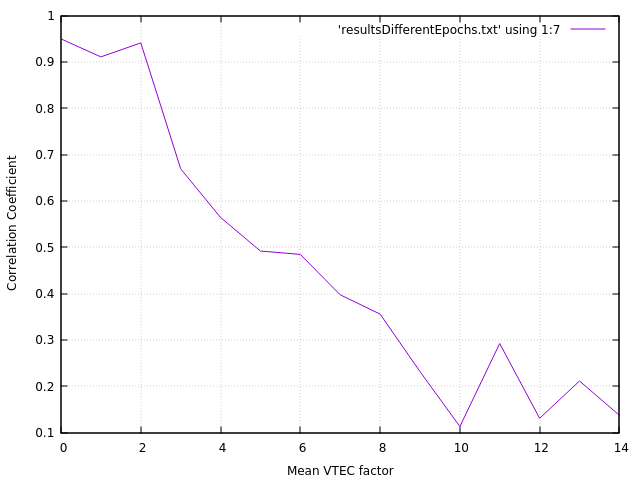
\includegraphics[width=\linewidth]{images/ch6/spikes/correlationDecrease.png}
		\caption{Correlation coefficient}
	\end{subfigure}
	\hfill
	\begin{subfigure}[b]{0.5\textwidth}
		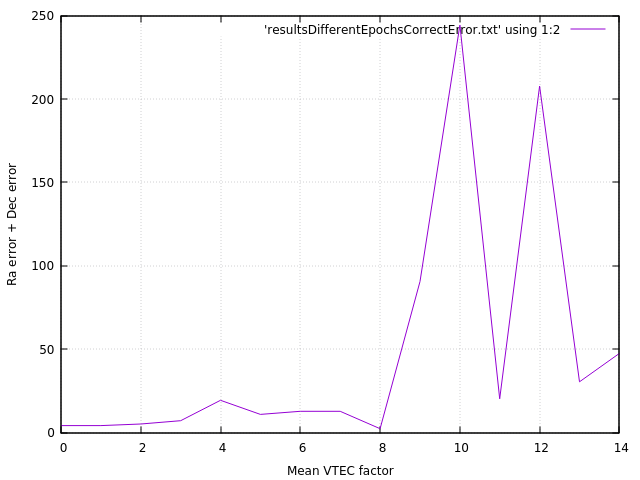
\includegraphics[width=\linewidth]{images/ch6/spikes/decreaseRangeError.png}
		\caption{Error of the estimated source}
	\end{subfigure}
	\caption{Correlation and error of the solution as the mean VTEC decreases}
	\label{fig:differentEpochs}
\end{figure}

As we can see, the correlation rapidly decreases from 1 (almost linear) to a negative coefficient. The error, on the other hand, doesn't experience much change for the first epochs but finally increases considerably. 

The fact that the error remains near 0 as the correlation rapidly decreases for the first epochs can be due to the fact that different location of the source reduces its effect on the  the estimated location with the highest correlation coefficient is still similar to that of the source. As the position of the source changes (the Sun in this case)  TODO: este parrafo

\subsection{Correlation}

As seen in the previous chapter, there exists a correlation between the VTEC value and the cosine of the solar-zenith angle. 

Once the moment of the flare is found, the aim of the algorithm is to study the correlation for each of the possible Suns and yield a fitness indicator for them. 

The main idea for the algorithm is that the higher the correlation, the more accurate the estimated location should be, compared to the Sun's real location. 

The results will be discussed in the last section of this chapter to see if the previous expectations are true.

\paragraph{Computation}

The correlation between two independent variables is defined as follows:

\begin{equation} \label{eq:coefficient}
r_{xy} = \frac{\sum(x_{i} - \bar{x})(y_{i} - \bar{y})}
{\sqrt{\sum(x_{i} - \bar{x})^{2}}
	\sqrt{\sum(y_{i} - \bar{y})^{2}}} \ \ \text{for} \ \ i \in (0, n)
\end{equation} \\

Although optimization is not the aim of this section, the previous formula would require passing the data twice: first to compute the mean of the cosine and VTEC and second to compute the coefficient itself. The formula can also be expressed as follows:

\begin{equation} \label{eq:singlePass}
r_{xy} = \frac{n\sum x_{i}y_{i} - \sum x_{i}\sum y_{i}}
{\sqrt{n\sum x_{i}^{2} - (\sum x_{i})^{2}}
	\sqrt{n\sum y_{i}^{2} - (\sum y_{i})^{2}}}  \ \ \text{for} \ \ i \in (0, n)
\end{equation} \\

With can be implemented with a single pass algorithm, as opposed to the former. Because of this we decided to initially start with this one.

\section{Algorithm}

The algorithm works as follows: the spike of VTEC value throughout the day is found by finding the epoch with the maximum mean VTEC of all IPPs for that epoch\footnote{The use of this method for finding the best epoch is discussed in chapter **** }.
The data is then filtered by that epoch (only the info of IPPs for that epoch will be used for the computations) and the algorithm starts considering possible Suns.

There are $360 * 180 = 64800$ possible Sun's. Thus, in order to test the algorithm, the factor \textit{STEP} is used which defines the step between the angles of possible Suns. The smaller the step, the more Suns will be considered. 

For each of these possible Suns, the VTEC value and the cosine of the solar-zenith angle ($\cos \chi$) are computed for every IPP in that epoch. Each of these Suns yields a data set with the aforementioned variables that can be plotted to obtain images such as the one studied at the end of the previous section. This two variables are used for computing the correlation coefficient for every considered Sun.

The following is the pseudocode for the brute force approach of the algorithm. Which returns the Sun that has yielded the highest correlation coefficient.

\begin{algorithm}
	\caption{Brute Force Approach}\label{pseudocodeBruteForce}
	\begin{algorithmic}[1]
		\Procedure{main}{}
		\State $\textit{epoch} \gets \text{findSpikeInData()}$ 
		\State $\text{filterDataByEpoch(\textit{epoch})}$
		\State $bestSun \gets nil$
		\For {$ra = 0;\ ra <= 360;\ ra += STEP$}
		\For {$dec = -90;\ dec <= 90;\ dec += STEP$}
		\State $currentSun \gets computeCorrelationPossibleSun(ra, dec)$
		\If {$currentSun.correlation > bestSun.correlation$} 
		\State $bestSun \gets currentSun$
		\EndIf
		\EndFor
		\EndFor
		\\
		\Return $bestSun$
		\EndProcedure
	\end{algorithmic}
\end{algorithm}

\clearpage

One thing that has to be taken into consideration is that all possible locations that have a declination of 90$^{\circ}$ or -90$^{\circ}$ yield the same results (figure \ref{fig:poles}).

\begin{figure}[!htb]
	\begin{subfigure}[b]{0.5\textwidth}
		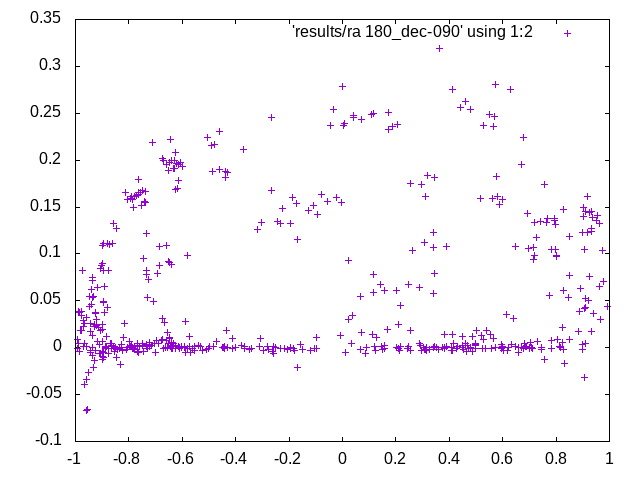
\includegraphics[width=\linewidth]{images/ch4/ra180_dec-090.png}
		\caption{ra=180$^{\circ}$, dec=-90$^{\circ}$}
	\end{subfigure}
	\hfill
	\begin{subfigure}[b]{0.5\textwidth}
		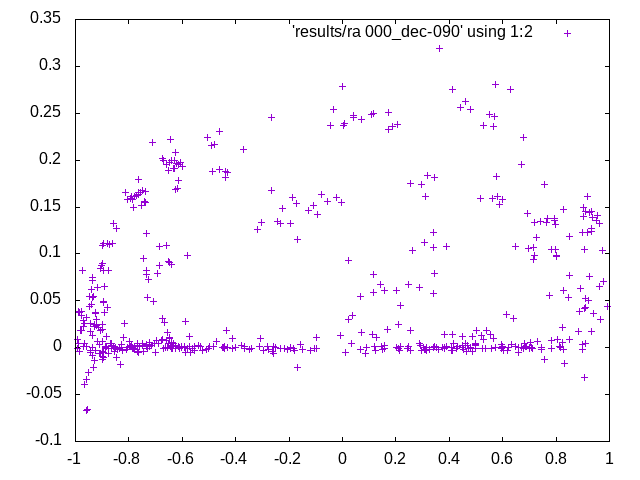
\includegraphics[width=\linewidth]{images/ch4/ra000_dec-090.png}
		\caption{ra=0$^{\circ}$, dec=-90$^{\circ}$}
	\end{subfigure}
	\caption{Two examples of possible Sun locations}
	\label{fig:poles}
\end{figure}

Using a \textit{diff} tool we can observe that although the data files used to plot the results \footnote{The data is $cos\chi$ for the X axis and VTEC for the Y axis} have different values, the resulting plots are exactly the same image.

This is due to the fact that declinations 90$^{\circ}$ and -90$^{\circ}$ correspond to the poles, when the Sun is directly on top or below the Earth, and therefore all possible right ascensions are exactly the same position.

\subsection{Implementation}

\paragraph{Finding the epoch}

The following loop traverses the data and computes the mean VTEC of each epoch, inserting it in a priority queue:

\begin{minipage}{\linewidth}
\begin{lstlisting}[language=c, caption=Finding a VTEC spike]
double epochIn, vtecIn, raIPPIn, latIPPIn;
int n = 0;

data >> epochIn >> vtecIn >> raIPPIn >> latIPPIn;
double totalEpochVTEC = vtecIn;
double previousEpoch = epochIn;
while (data >> epochIn >> vtecIn >> raIPPIn >> latIPPIn) {
	totalEpochVTEC += vtecIn;
	n++;
	if (previousEpoch != epochIn) {
		insertCandidate(previousEpoch, totalEpochVTEC/n);
		previousEpoch = epochIn;
		totalEpochVTEC = 0;
		n = 0;
	}
}
\end{lstlisting}
\end{minipage}


\paragraph{Iterating over the possible Suns}

The main loop of the algorithm considers for each possible declination, each possible right ascension (taking into consideration the special case of the poles) and uses said declination and right ascension to compute the correlation coefficient, saving the one with the max value.

\begin{minipage}{\linewidth}
\begin{lstlisting}[language=c, caption=Main loops]
for (int dec = -90; dec <= 90; dec += step) {
	if (dec != -90 and dec != 90) {
		for (int ra = 0; ra <= 360; ra += step) {
			pearsonCoefficient = computeCorrelation(&ra, &dec);
			if (pearsonCoefficient > maxCoefficient) {
				maxCoefficient = pearsonCoefficient;
				location = "[" + to_string(ra) + ", " + to_string(dec) + "]";
			}
		}
	}
	else {
		int ra = 0;
		pearsonCoefficient = computeCorrelation(&ra, &dec);
		if (pearsonCoefficient > maxCoefficient) {
			maxCoefficient = pearsonCoefficient;
			location = "[" + to_string(ra) + ", " + to_string(dec) + "]";
		}
	}
}
\end{lstlisting}
\end{minipage}

\paragraph{Computing the correlation}

This is the main code of the Fortran function \textit{computeCorrelation(ra, dec)} called for every possible \textit{(ra, dec)} pair considered in the previous loop. Other auxiliary functions appear in the \textit{computeCorrelation(ra, dec)} function such as \textit{openFile()} (opens the file for reading) or \textit{toRadian()} (converts the degrees from the input to radians, used by Fortran's trigonometric functions). These functions are not included for readability.

\textit{computeCorrelation(ra, dec)} reads every line of the file that contains the information of the IPPs filtered by the found epoch and computes both the solar-zenith angle and the VTEC using the same procedures seen in the previous chapter:

\begin{lstlisting}[language=Fortran, caption=Correlation computation]
double precision function traverseFile (raSunIn, decSunIn)
	implicit none
	integer, intent(in) :: raSunIn, decSunIn
	double precision :: raIPP, decIPP, raSun, decSun, mapIon, d2Li, cosX, vtec
	double precision :: sumx = 0, sumy = 0, sumxy = 0, sumx2 = 0, sumy2 = 0
	double precision :: rxyPearson
	integer :: i = 0
	
	sumx = 0
	sumy = 0
	sumxy = 0
	sumx2 = 0
	sumy2 = 0
	i = 0
	
	raSun = raSunIn
	decSun = decSunIn
	raSun = toRadian(raSun)
	decSun = toRadian(decSun)
	call openFile()
	do while (1 == 1)
		read (1, *, end = 240) raIPP, decIPP, mapIon, d2Li
		raIPP = toRadian(raIPP)
		decIPP = toRadian(decIPP)
		vtec = estimateVTEC(mapIon, d2Li)
		cosx = computeSolarZenithAngle (raIPP, decIPP, raSun, decSun)
		if (cosx > CORRELATION_THRESHOLD) then
			call updateCorrelationParameters (cosx, vtec, sumx, sumy, sumxy, sumx2, sumy2)
			i = i + 1
		end if	
	end do
	240 continue
	close(1)
	rxyPearson = computePearsonCoefficient(i, sumx, sumy, sumxy, sumx2, sumy2)
	return
end function traverseFile
\end{lstlisting}

As can be seen in the code, the line (IPP) is only considered if $\cos\chi$ is higher than a \textit{"correlation threshold"} ($-0.1^{\circ}$ in this case). This is done because we want to study only the "part" of the ionosphere where the Sun is having an effect. This can be seen in figure \ref{fig:solar-zenith-angle}, where we observed that the VTEC value remained the same from $\cos\chi = -1$ (180$^{\circ}$) to $\cos\chi = 1$ (0$^{\circ}$).

Once the two variables are computed (\textit{vtec} and \textit{cosx}, in the code), the necessary summations for computing the correlation are updated each iteration:

\begin{itemize}
	\item $\sum x_{i}$ and $\sum y_{i}$
	\item $\sum x_{i}y_{i}$
	\item $\sum x_{i}^{2}$ and $\sum y_{i}^{2}$
\end{itemize}

The following code updates this summations:

\begin{lstlisting}[language=Fortran, caption=Function to update the necessary summations]
subroutine updateCorrelationParameters (x, y, sumx, sumy, sumxy, sumx2, sumy2)
	implicit none
	double precision, intent(in) :: x, y
	double precision :: sumy, sumy2, sumxy, sumx2, sumx

	sumx = sumx + x
	sumy = sumy + y
	sumxy = sumxy + x*y
	sumx2 = sumx2 + x*x
	sumy2 = sumy2 + y*y

	return
end subroutine updateCorrelationParameters
\end{lstlisting}

Finally, once all the IPPs have been processed, the previous summations are used to compute the Pearson Correlation Coefficient using equation \ref{eq:singlePass}, the value the function returns to the C++ code.

\begin{lstlisting}[language=Fortran, caption=Function to compute the correlation coefficient using the summations]
double precision function computePearsonCoefficient (n, sumx, sumy, sumxy, sumx2, sumy2)
	implicit none
	integer, intent(in) :: n
	double precision, intent(in) :: sumx, sumy, sumxy, sumx2, sumy2 
	double precision :: rxyPearsonCoefficient

	numerator = n*sumxy - sumx*sumy
	denominator = sqrt(n*sumx2-sumx*sumx)*sqrt(n*sumy2-sumy*sumy)

	rxyPearsonCoefficient = numerator/denominator
	return
end function computePearsonCoefficient
\end{lstlisting}

\paragraph{Compiling}

The C++ and Fortran compilers allow us to compile both languages and their libraries together. With this, the main part of the algorithm can be implemented using C++ which can then call Fortran for the parts that require heavy numerical computation.

This can be done by compiling the object of the Fortran code using the $-c$ flag, and then linking it with the C++ code using the $-lgfortran$ flag so that the standard Fortran libraries are included: \\

\textit{gfortran fortranFunctions.f90 -c -o functions.o}
	
\textit{g++ functions.o bruteForce.cc -o bruteForce.x -lgfortran}

\subsection{Results}

Executing the algorithm with a STEP of 10$^{\circ}$, this is the output of the execution:

\begin{lstlisting}[caption=Brute force approach algorithm output]
[C++: Finding a spike in the VTEC distribution]
	-> Spike found: 11.05
[AWK: Filtering all data by best epoch: 11.05]
[C++ -> Fortran: Finding the Person coefficients for possible Suns]
	-> Input degree step: 10
[631 possible Suns considered]
[C++: Results]
	-> Largest correlation coefficient: 0.926959
	-> Estimated Sun's location: [ra=210, dec=-10]
\end{lstlisting}

As we can see, the possible Sun with the highest correlation coefficient (0.9269) has a location with a right ascension of 210$^{\circ}$ and a declination of -10$^{\circ}$. Considering that for the epoch we are working with the Sun position was $212.338^{\circ}$ and $-13.060^{\circ}$ as the right ascension and declination, respectively, we can see that the estimated Sun's location returned by the algorithm is close to the real one, using a step of 10$^{\circ}$.

It can be interesting to see how the computation time grows as more precision is demanded from the algorithm, and if the precision of the results does as well. The following table shows this relation for some input cases:

\begin{table}[h!]
	\centering
	\def\arraystretch{1.2}
	\begin{tabular}{|c c c c c|} 
		\hline
		Step & Considered Suns & Correlation coefficient & Estimated location & Execution time \\ [0.5ex] 
		\hline\hline
		100 & 5 & 0.695358 & [ra=200, dec=10] & 867ms \\
		\hline 
		50 & 25 & 0.695358 & [ra=200, dec=10] & 303ms \\
			\hline 
		25 & 106 & 0.866293 & [ra=225, dec=-15] & 820ms \\
			\hline 
		12 & 436 & 0.92287 & [ra=216, dec=-6] & 956ms \\
			\hline 
		6 & 1771 & 0.934663 & [ra=216, dec=-12] & 1s 385ms \\
			\hline 
		3 & 7141 & 0.937349 & [ra=213, dec=-12] & 7s 169ms \\
			\hline 
		1 & 64621 & 0.939114 & [ra=214, dec=-11] & 1m 9s 564ms \\
		\hline 
	\end{tabular}
	\caption{Results}
\end{table}

As we can see this approach provides the expected results, but has a large computational complexity that increases with the precision we demand. 

Furthermore, we can see that a problem appears: in the last two cases there is an increase in the correlation coefficient as expected, but the estimated Sun location does not improve, it is actually less accurate than the previous one.

In the next chapter, an optimization is presented for the algorithm to perform these computations, aiming to reduce its complexity.
\chapter{Decreasing search range method}

\textbf{falta revisar seccion linear fit}

In the previous chapter we saw that the BGSEES algorithm for detecting the location of an EUV source (in this case, the Sun) is possible with a first, brute force approach. Here, the algorithm is studied in more detail considering a different method aiming to increase its precision and reduce its computational complexity.

\section{Decreasing the range of the search}

As we saw in the previous chapter, to increase the precision of the algorithm, the \textit{step} with which we iterate over the possible angles (right ascension and declination) is reduced. This causes more possible Suns to be considered. For example, with a step of one degree, we consider all possible right ascensions [0,360] and declinations [-90,90]: $360*180 = 64800$ Suns, minus the $2*360 - 2 = 718$ right ascensions we do not consider\footnote{We do not consider the 360 right ascensions of the two poles (-90 and 90), hence 2*360, but we do consider the two poles themselves (with any valid right ascension)} because as we have seen right ascensions for declinations of -90 and 90 are the same location.

We want to have the highest precision possible without having to consider all $64800 - 718 = 64082$ possibilities by progressively reducing the search range.

This first method works as follows: the entire possible range is considered with a large starting step (e.g 60). Once the best Sun is found within this range, the precision is increased (the step is decreased) and the search range is reduced. This way the precision is increased but the number of considered possibilities remains similar each iteration of the algorithm.

\section{Pseudocode}

The following is the pseudocode\footnote{The code for the special cases of -90 and 90 degree declinations is not included for more readability. It is included in the implementation, in the following section.} for the algorithm using this method:

\begin{algorithm}
	\caption{Search range decrease}\label{searchRangeDecrease}
	\begin{algorithmic}[1]
		\Procedure{main}{}
		\State $\textit{epoch} \gets \text{findSpikeInData()}$
		\State $\text{filterDataByEpoch(\textit{epoch})}$
		\State $bestSun \gets nil$
		\State $r \gets \text{defaultRange()}$
		\For {$step = initStep; step >= min; step\ /= 2$}
		\For {$ra = r.lowerRa;\ ra <= r.upperRa;\ ra += step$}
		\For {$dec = r.lowerDec;\ dec <= r.upperDec;\ dec += step$}
		\State $currentSun \gets computeCorrelationPossibleSun(ra, dec)$
		\If {$currentSun.correlation > bestSun.correlation$}
		\State $bestSun \gets currentSun$
		\State $r \gets \text{newRange(\textit{bestSun, step})}$
		\EndIf
		\EndFor
		\EndFor
		\EndFor
		\\
		\Return $bestSun$
		\EndProcedure
	\end{algorithmic}
\end{algorithm}

\section{Implementation}

This first piece of code is the main loop of the method, which starts with a default range of ra=[0, 360], dec=[-90, 90] and is reduced every iteration based on the current best Sun's estimated location.

Furthermore, because an increase in the precision of the tested location does not necessarily imply an improvement in the solution, the new candidate is inserted into a \textit{priorityQueue} ordered by the coefficient to assure that the method returns the best one found throughout the entire execution (it is inserted into a priority queue for debugging purposes, but simply saving the best solution would be more efficient).

\begin{minipage}{\linewidth}
	\begin{lstlisting}[language=c, caption=Decreasing the range and increasing the precision]
void TraverseGlobe::decreasingSTEP() {
	int rangeSize = 3;
	int initStep = 60;
	sourceInfo currentSun;
	searchRange range = setRange(currentSun, true, initStep, rangeSize);
	for (double step = initialStep; step >= 0.5; step /= 2) {
		currentSun = considerPossibleSuns(step, range, plotData);
		bestSuns.push(currentSun);
		range = setRange(currentSun, false, step, rangeSize);
	}
}\end{lstlisting}
\end{minipage}

The \textit{setRange} function sets a new range based on the estimated location that depends on the precision used for the values and checks that valid range values are returned.

\begin{minipage}{\linewidth}
	\begin{lstlisting}[language=c, caption=Setting the new range based on the estimated source location]
searchRange setRange(sourceInfo sun, bool defaultR, double step, int rangeSize) {
	searchRange r;
	if (defaultR) {
		r.lowerRa = 0;
		r.upperRa = 360;
		r.lowerDec = -90;
		r.upperDec = 90;
	}
	else {
		double rRange = step*rangeSize;
		double dRange = step*rangeSize;
		r.lowerRa = sun.ra - rRange >= 0 ? sun.ra - rRange : 0;
		r.upperRa = sun.ra + rRange <= 360 ? sun.ra + rRange : 360;
		r.lowerDec = sun.dec - dRange >= -90 ? sun.dec - dRange : -90;
		r.upperDec = sun.dec + dRange <= 90 ? sun.dec + dRange : 90;
	}
	return r;
}\end{lstlisting}
\end{minipage}

Finally, the \textit{considerPossibleSuns} function has the same functionality as the one from the previous chapter, it iterates over the possible locations, this time, however, it does so over the given range, rather than just the default one.

The names of the lower and upper bound variables have been changed (\textit{uRa} instead of \textit{upperRa}, for example) for readability.

\begin{minipage}{\linewidth}
	\begin{lstlisting}[style=myCStyle, caption=Iterating over possible locations within the given range]
sourceInfo considerPossibleSuns(double step, searchRange range) {
	FortranController fc;
	double pearsonCoefficient;
	int i = 0;
	sourceInfo bestSun;
	bestSun.coefficient = -23;
	bestSun.location = "salu2";

	for (double dec = range.lDec; dec <= range.uDec; dec += step) {
		if (dec != -90 and dec != 90) {
			for (double ra = range.lRa; ra <= range.uRa; ra += step) {
				pearsonCoefficient = fc.computeCorrelation(&ra, &dec);
				if (pearsonCoefficient > bestSun.coefficient) {
					bestSun.coefficient = pearsonCoefficient;
					bestSun.ra = ra;
					bestSun.dec = dec;
				}
			}
		}
		else {
			//Do only once
			double ra = 0;
			pearsonCoefficient = fc.computeCorrelation(&ra, &dec);
			if (pearsonCoefficient > bestSun.coefficient) {
				bestSun.coefficient = pearsonCoefficient;
				bestSun.ra = ra;
				bestSun.dec = dec;
			}
		}
	}
	return bestSun;
}\end{lstlisting}
\end{minipage}

Finally, the \textit{computeCorrelation} calls the Fortran code (the same used in the Brute Force chapter) to compute the correlation

Figure \ref{fig:consideredSolutions} is a visual representation of how the algorithm works. The X and Z axis are the possible right ascensions
and declinations (the possible solutions to our problem) and the Y axis is the correlation coefficient.

\begin{figure}[!htb]
	\begin{centering}
		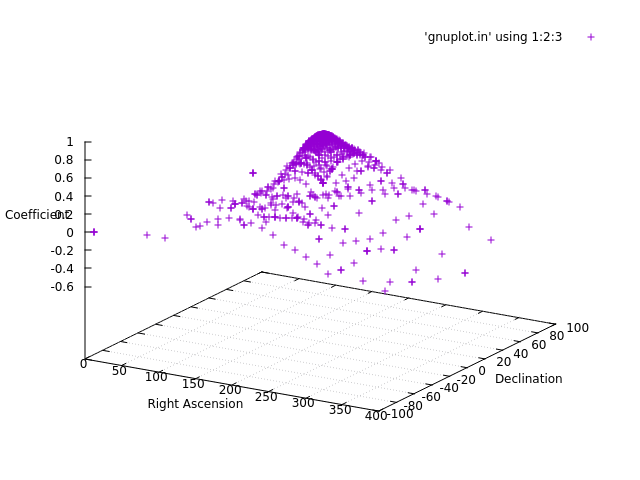
\includegraphics[width=0.5\linewidth]{images/ch6/hillClimbing/resultsAll.png}
		\caption{All visited candidates of the solution space}
		\label{fig:consideredSolutions}
	\end{centering}
\end{figure}

As we can see in the plot, as we increase the precision of the search, the range decreases, this can be seen because each point
of the plot is each of the locations considered by the algorithm: the density of considered solutions increases as the algorithm gets closer to the local maxima, the correct solution we are looking for.

Another change that could be done to improve this method's performance would be to adopt a sort of \textit{"Dynamic Programming"} strategy in order to avoid repeated calculations (the new range will always be inside the previous range). However, the problem is that because we are dealing with a different precision for the right ascension and declination values every loop, the algorithm is not working with the exact same value.

\section{Linear fitting: discarding outliers}

In the previous chapter we used a simple method to discard outliers for the VTEC value (using a cutoff value between -0.7 and 0.7). However, another approach to discard outliers was possible: linear fitting. 
The aim is to find the line that fits best the relation between both variables (cosine and VTEC) by means of linear regression to discard samples that do not fit in it.

We can see that this procedure has been used before in figure \ref{fig:halloweenPaper} from the paper \textit{"GNSS measurement of EUV photons flux rate during strong and mid solar flares"}\cite{hernandez2012gnss}.

Manuel Herández-Pajares, the author, provided the Fortran program that performs this computation. After integrating it with the rest of the code, figure \ref{fig:linearFit} shows the result of testing it with the flare used in the previous chapter:

\begin{figure}[!htb]
	\begin{centering}
	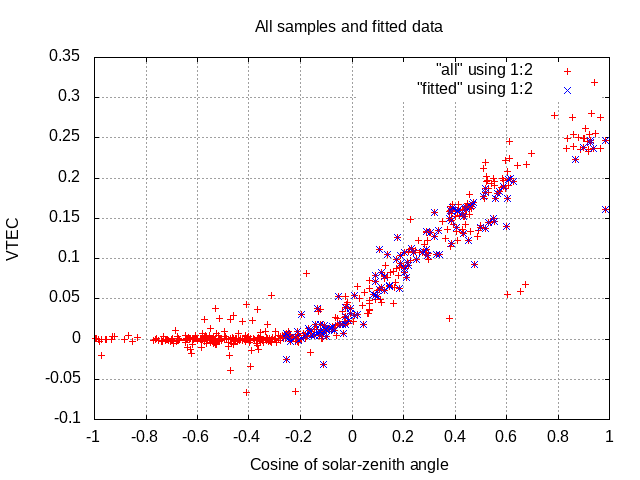
\includegraphics[width=0.5\linewidth]{images/ch6/linearFit/resultAll.png}
		\caption{All data (red) and fitted samples (blue)}
		\label{fig:linearFit}
	\end{centering}
\end{figure}

The main problem of this method without it, the correlation could be calculated in a single pass of the data. Now, on the other hand, the algorithm needs multiple iterations: first, the solar-zenith angle cosine for each IPP is calculated; then, the outliers are discarded, and finally, the filtered data is traversed one last time to compute the correlation.

Here is the new code in order to compute the correlation for each possible location:

\begin{minipage}{\linewidth}
\begin{lstlisting}[language=C++, caption=Discarding outliers and computing the correlation]
double computeCorrelation(double* ra, double* dec) {
	FileManager fileManager;
	int sigma = 1;
	int iterations = 6;
	computecosinesofcurrentsourcefortran_(ra, dec);
	fileManager.discardOutliersLinearFitFortran(sigma, iterations);
	return computecorrelationfortran_(ra, dec);
}\end{lstlisting}
\end{minipage}

As we can see, the data is traversed \textbf{at least} 3 times now (more depending on the number of iterations).

\section{Results}

Executing the algorithm with both methods for discarding outliers using the data set from the previous chapter we obtain:

\begin{minipage}{\linewidth}
\begin{lstlisting}[language=, caption=Decreasing range using a cutoff value for outliers]
Estimation error: 1.86776 degrees
Execution time: 1.07601 seconds
\end{lstlisting}
\end{minipage}

As we can see, the algorithm provides a better estimation than the brute force approach. Which took more than minute yielding a result with a precision of 1 degree.

Testing the algorithm using the linear fit approach to discard outliers we obtain the following result:

\begin{minipage}{\linewidth}
\begin{lstlisting}[caption=Decreasing range using linear fit for outliers]
Estimation error: 3.57674 degrees
Execution time: 37.5578 seconds 
\end{lstlisting}
\end{minipage}

For this data set in particular, the solution has a similar error (although the linear fit version does not improve with respect to the one with a basic filter) and the execution time is increased considerably. This comparison will be studied in more detail in the \textit{Results} chapter, where different data sets will be used. \\

Seeing the increase in computational complexity of this method when discarding outliers using linear fitting, we decided to focus on a different method that would rely only on the data itself, instead of considering the many possible locations of the source.

\chapter{Least Squares method}

As we have seen in previous chapters the overall process to determine the location of the source is studying the correlation between the VTEC value and the solar-zenith angle (or source-zenith angle, speaking in general terms) for a possible location.

That is, for an IPP with a location and an associated VTEC value, given the location of a possible source, compute the cosine between them, and see that the closer the cosine to 1 (or 180º), the higher the VTEC value.

The idea that we wanted to test with this method was finding the location of the source by performing the inverse operation: having the VTEC, location of the IPP and correlation (1, assuming a near-linear correlation), obtaining the source's right ascension and declination.

\section{The equation system}

The source-zenith cosine between the source and the IPP was computed using the following equations:

\begin{equation} \label{eq:61}
unitVectorIPP =
\begin{bmatrix}
X' \\
Y' \\
Z'
\end{bmatrix}
=
\begin{bmatrix}
\cos\delta_{g} * \cos\alpha_{g} \\
\cos\delta_{g} * \sin\alpha_{g} \\
\sin\delta_{g}
\end{bmatrix}
\end{equation}

\begin{equation} \label{eq:62}
unitVectorSource =
\begin{bmatrix}
X \\
Y \\
Z
\end{bmatrix}
=
\begin{bmatrix}
\cos\delta_{s} * \cos\alpha_{s} \\
\cos\delta_{s} * \sin\alpha_{s} \\
\sin\delta_{s}
\end{bmatrix}
\end{equation}

\begin{equation} \label{eq:63}
\cos \chi = unitVectorIPP \cdot unitVectorSource
\end{equation}\\

Having the VTEC and source-zenith cosine, we could find the correlation of the two variables, expecting that the real source would yield a near-linear correlation.

Visually, we can see the relation between VTEC and the computed cosine in figure \ref{fig:solar-zenith-angle}, obtained in chapter 3 when studying the a specific case for the Sun.

\begin{figure}[!htb]
	\begin{centering}
		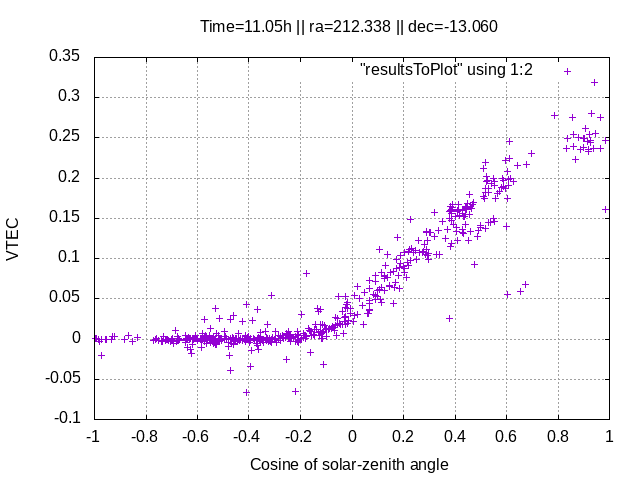
\includegraphics[width=0.5\linewidth]{images/ch4/resultSunTest.png}
		\caption{VTEC as a function of the solar-zenith angle's cosine}
		\label{fig:solar-zenith-angle}
	\end{centering}
\end{figure}

As we have previously seen for this case, there appears to be a linear relation starting around $\cos \chi = -0.1$ between the two studied parameters. Therefore, we could define this linear relation as a \textbf{straight line} ($y = mx + b$) by expressing the estimated VTEC value ($\Delta V$) as a function of the source-zenith cosine (\ref{eq:linearRelation}).

\begin{equation} \label{eq:linearRelation}
\Delta V = a\cos \chi + b
\end{equation}

Because the cosine is computed using the previous equations (\ref{eq:61}, \ref{eq:62}, \ref{eq:63}). It can be expressed as follows:

\begin{equation} \label{eq:cosine}
\cos \chi = XX' + YY' + ZZ'
\end{equation}

Where $X'$, $Y'$, $Z'$ are the components of the IPP's unit vector obtained from equation \ref{eq:61}, and $X$, $Y$, $Z$ are the unknowns of our equation: the components of the source's unit vector, which could be used to easily find the right ascension and declination of the source by using trigonometric operations.

However, finding the value of this unknowns is the difficult part of this method. Taking the cosine as \ref{eq:cosine} we can express the linear function as:

\begin{equation} \label{eq:substitute}
\Delta V = aXX' + aYY' + aZZ' + b
\end{equation}

Because $a$ and $b$ are unknowns as well as $X$, $Y$ and $Z$, we can group them as follows:

\begin{equation} \label{eq:newNames}
\Delta V = \alpha X' +  \beta Y' +  \gamma Z' + b
\end{equation}

Our aim now would be to solve the previous equation, but then we would need to obtain only the values of $X$, $Y$ and $Z$. We can see that:

\begin{equation} \label{eq:elTrucoDelAlmendruco}
\sqrt{\alpha^{2}+\beta^{2}+\gamma^{2}} = \sqrt{a^{2}(X^{2}+Y^{2}+Z^{2})} = \sqrt{a^{2}} = a
\end{equation}

Because $X$, $Y$ and $Z$ are the components of a unit vector\footnote{$\sqrt{(X^{2}+Y^{2}+Z^{2})} = 1$}. The previous allows us to, once we know the values of $\alpha$, $\beta$ and $\gamma$, obtain $X$, $Y$ and $Z$ by doing:

\begin{equation} \label{eq:iso}
\frac{\alpha}{\sqrt{\alpha^{2}+\beta^{2}+\gamma^{2}}} = \frac{\alpha}{a} = \frac{aX}{a} = X
\end{equation} \\

In our data we can find, for each IPP: $\Delta V$, $X'$, $Y'$, $Z'$ (because we have the right ascension and declination of the point).

For each of these IPPs, we have an equation of the form $\Delta V = \alpha X' +  \beta Y' +  \gamma Z' + b$ and, therefore, we have an overdetermined system of equations, with more equations (unknown, depends on the input data) than variables (four: $\alpha$, $\beta$, $\gamma$ and $b$)

Knowing how to obtain $X$, $Y$ and $Z$ from $\alpha$, $\beta$ and $\gamma$, we can now focus on solving the system of equations to obtain the latter unknowns .

Because we have an overdetermined system of equations, the solution can be approximated using the Least Squares approach. The system can be represented in matrix form $y = AX$ as follows:

\begin{equation} \label{eq:matrixSystem}
\begin{bmatrix}
\Delta V_{0} \\
\Delta V_{1} \\
. \\
. \\
. \\
\Delta V_{n}
\end{bmatrix}
=
\begin{bmatrix}
X'_{0} & Y'_{0} & Z'_{0} & 1 \\
X'_{1} & Y'_{1} & Z'_{1} & 1 \\
. & . & . & .\\
. & . & . & .\\
. & . & . & .\\
X'_{n} & Y'_{n} & Z'_{n} & 1 \\
\end{bmatrix}
\begin{bmatrix}
\alpha \\
\beta \\
\gamma \\
b \\
\end{bmatrix}
\end{equation}

This way, X can be obtained by means of the least squares estimate equation:

\begin{equation}
	X = (A^{T}A)^{-1}A^{T}y
\end{equation}

\section{Pseudocode}

\section{Implementation}

When

One of the main advantages of this method over the others is that we don't need to compute the correlation, that it is, discard outliers. (o si????)

\chapter{Other methods}

Here other possible optimizations are considered that could be used to, in the future, extend the algorithm and perhaps improve its performance and accuracy.

\section{Hill Climbing}

explicar que no es hill climbing exactamente, algo mas simple rollo greedy 
Using the previous optimization we can see a plot of all the possibilities the algorithm considers:

\begin{figure}[!htb]
	\begin{centering}
		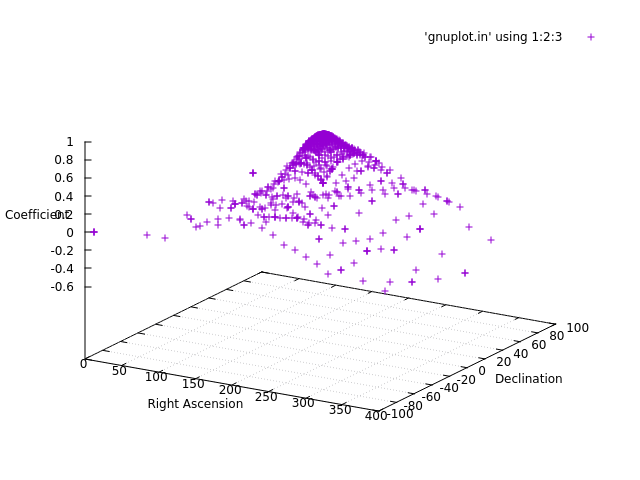
\includegraphics[width=0.5\linewidth]{images/ch6/hillClimbing/resultsAll.png}
		\caption{All visited candidates of the solution space}
		\label{fig:solutionSpace}
	\end{centering}
\end{figure}

As we can see in the previous figure, there appears to be a "hill" (our solution) so an attempt to solve the problem using a \textit{Hill Climbing} approach was also considered.

While not exactly Hill Climbing, a simple greedy algorithm was implemented as a first attempt to test if this method could yield good results:

\begin{minipage}{\linewidth}
	\begin{lstlisting}[language=c, caption=Hill Climbing]
	// Starting position
	sourceInfo current;
	current.ra = 160;
	current.dec = -20;
	int i = 0;
	// Loop with limit or until no progress can't be made
	while (++i < 100) {
		vector<sourceInfo> candidates = getNeighbourList(current);
		sourceInfo newCandidate = getBestCandidate(candidates);
		if (newCandidate < current) {
			break;
		}
		current = newCandidate;
	}
	\end{lstlisting}
\end{minipage}

The following figure shows the results of the execution for two different starting states. For both of them, the algorithm ran until it couldn't progress any further (wasn't interrupted by the iteration limit). The plots contain both the possibilities considered by the decrease range method (in purple, the same plot as \ref{fig:solutionSpace}) and the path taken by the Hill Climbing method (in green).

\begin{figure}[!htb]
	\begin{subfigure}[b]{0.5\textwidth}
		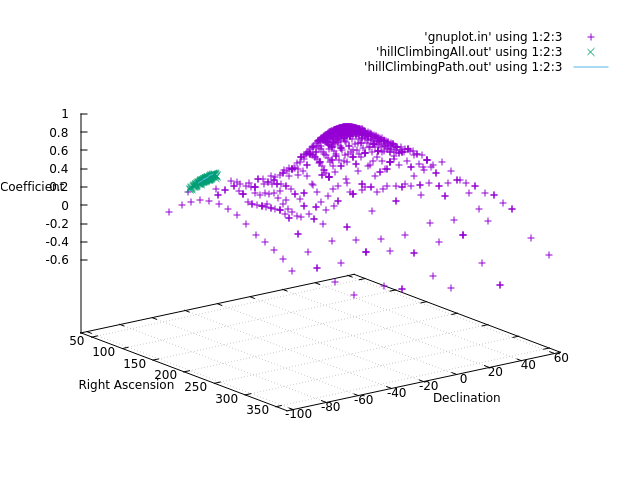
\includegraphics[width=\linewidth]{images/ch6/hillClimbing/resultsPathBad.png}
		\caption{Start: ra=100$^{\circ}$, dec=-60º}
	\end{subfigure}
	\hfill
	\begin{subfigure}[b]{0.5\textwidth}
		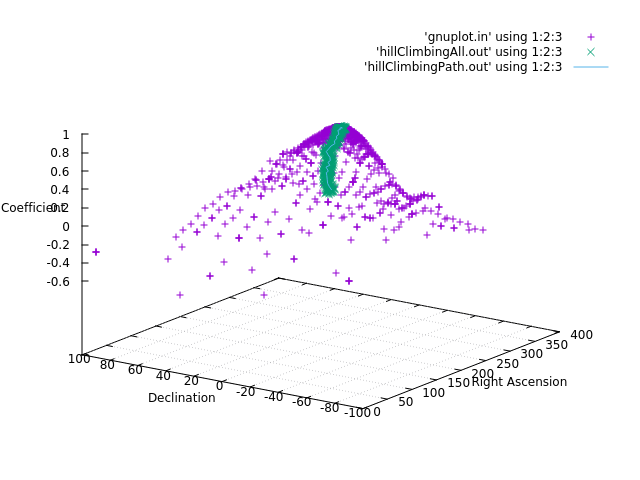
\includegraphics[width=\linewidth]{images/ch6/hillClimbing/resultsPathGood.png}
		\caption{Start: ra=160º, dec=-20º}
	\end{subfigure}
	\caption{Paths taken by the Hill Climbing algorithm}
	\label{fig:hillClimbingPaths}
\end{figure}

Visually, we can see that the number of considered possibilities is inferior and the top is reached for case (b), but a problem appears: \textbf{a local maxima}.

If we take a starting right ascension of 160º and a declination of -20º, the algorithm takes a path that gets to the top of our solution, yielding similar results to the previous, decrease range method.

However, with a starting right ascension of 100º and a declination of -60º, the algorithm finds a local maxima on its way and can't progress to the real best solution.

As a result, we can't rely on the Hill Climbing approach for all cases, considering that local maxima may exist for our type of problem. Because of this, another possibility would be to use the Simulated Annealing algorithm so that we can explore other parts of the solution space and find other paths that might lead to our desired solution, instead of only.

\section{Simulated Annealing}

\section{OpenMP}

Explicar OpenMP

\section{Discarding the Sun hemisphere}

So far the algorithm has been studied for the case of the Sun, as it is a source that should be detected more easily than far-away stars. 

The main idea is that the algorithm should detect extraterrestrial EUV sources (if possible) other than the Sun. it follows that it should, before any other computations, discard the Sun hemisphere based on the current Sun location. The greater impact of the Sun's radiation due to its proximity would blind the algorithm from detecting sources that may be having an effect on that hemisphere because of the noise.


bla bla bla

This will be used in the next chapter, in which the presented methods will tested with flares from the Sun and far-away stars.
\chapter{Results}

In this chapter we will study different data sets using the two presented methods for the \textit{BGSEES} algorithm: the \textbf{Least Squares} and \textbf{Decrease Range} method. 

The aim of the chapter is to test them against each other and using different parameters to see which method yields the best result

The algorithm is tested using data from both Solar flares and flares from far-away stars. Because the day hemisphere has to be discarded in order to study far-away stars (because of the Sun's effect on the ionosphere), the first section will study examples of flares originating from the Sun and the second those from outside the Solar System.

\section{Sun}

For the solar flares, the ti files of days when a flare had taken place were used to compare the results. The data was filtered around the time of the flare (30 minutes before and after, if there was an exact moment in time).
 
Below is the list of times (\textit{year.day.seconds}) of the different flares we studied. The seconds are either an exact moment in time or a range used in the plots of the papers the flares are listed in.

Flares listed in \textit{"GNSS measurement of EUV photons flux rate during strong and mid solar flares"}\cite{hernandez2012gnss}

\begin{itemize}
	\item 2003.301.39777
	\item 2003.308.71000-71100
	\item 2005.020.24200-24400
	\item 2006.340.67300-67500
	\item 2011.210.44134
	\item 2011.216.13908
\end{itemize}

And those listed in \textit{"GPS as a solar observational instrument: Real-time estimation of EUV photons flux rate during strong, medium, and weak solar flares"}\cite{singh2015gps}

\begin{itemize}
	\item 2001.334.3700-4000
	\item 2001.347.51800-52200
	\item 2002.196.72240
	\item 2004.204.27800-28000
	\item 2004.310.41370
	\item 2004.313.52500
	\item 2005.258.30990
	\item 2012.066.4400-4700
	\item 2012.130.50600-51000
	\item 2012.297.11600-12000
	\item 2013.310.35970
\end{itemize}

To perform this study, the best epoch within the given range is found using the mean VTEC, as shown in chapter 5. The data is then filtered using this epoch and the algorithm is executed using the necessary parameters, the studied factors are:

The \textbf{execution time} of the algorithm and the \textbf{absolute error} of the estimation, obtained by computing the angle between correct Sun position\footnote{The correct Sun position at that moment is obtained from the data, it is one of the many fields the ti files contain} and the estimated location, using the same operations we've used in previous chapters to compute the angle. 

The ti files that contain data for the entire day are filtered using this bash script, which has a list with the information of each file to be filtered: the name of the original file and the upper and lower limits of time. It then filters each file using a simple AWK one-line script that checks the field with the time:

\begin{minipage}{\linewidth}
	\begin{lstlisting}[language=Bash, caption=Filtering the ti file]
	#!/bin/bash	
	
	strings=(
	'ti.2003.301.gz,10,11.5'
	)
	for i in "${strings[@]}"; do
	
	done
	
	\end{lstlisting}
\end{minipage}

The study is divided in three categories, based on the method used to discard outliers from the input data:

\begin{itemize}
	\item Using the data from \textbf{all IPPs} without filtering out any outliers
	\item Using a simple \textbf{cutoff value} for the VTEC
	\item Using \textbf{linear fit} for the Decreasing Range method to discard outliers and \textbf{multiple iterations} for the Least Squares method to try to improve the solution, both explained in their respective chapters.
\end{itemize}

\section{Using all available data}

The main problem of this method is that outliers that are far from the sample make the mean computation unstable, leading to using incorrect epochs.

\subsubsection{Decreasing range}

\begin{table}[h!]
	\centering
	\def\arraystretch{1.2}
	\begin{tabular}{|c c c|} 
		\hline
		Data set & Total estimation error & Time \\ [0.5ex] 
		\hline\hline
		X17.2  & 4.09113 & 0.79132 \\
		\hline
		Other & 181.501 & 5.17015 \\
		\hline\hline
		Total & 4.09113 & 6565 \\
		\hline
	\end{tabular}
	\caption{Results for different epochs}
\end{table}

\subsubsection{Least Squares}

\begin{table}[h!]
	\centering
	\def\arraystretch{1.2}
	\begin{tabular}{|c c c c c|} 
		\hline
		Data set & Right Ascension Error & Declination Error & Total estimation error & Time \\ [0.5ex] 
		\hline\hline
		X17.2 & 3.31917 & 0.771964 & 4.09113 & 0.79132 \\
		\hline
		Other & 97.1888 & 84.3119 & 181.501 & 5.17015 \\
		\hline\hline
		Total & 4343 & 5454 & 4.09113 & 6565 \\
		\hline
	\end{tabular}
	\caption{Results for different epochs}
\end{table}

\subsubsection{Discussion}

As we can see

\subsection{Direct VTEC filter}

This is the first method used in the brute force approach that yielded results very similar to the real location of the Sun, but it does not work well with other data sets.

The filter is done using a cutoff value for the VTEC when the data is first filtered

Different cutoff values are studied to see if this is a reliable method, as it simplifies the overall computation of the algorithm considerably.

\subsection{Discarding outliers}

\subsubsection{Decreasing range: linear fit}

\subsubsection{Least Squares: Iteration}

We iterate bla bla bla

\begin{table}[h!]
	\centering
	\def\arraystretch{1.2}
	\begin{tabular}{|c c c c c c|} 
		\hline
		Data set & Iterations & RA Error & Declination Error & Total estimation error & Time \\ [0.5ex] 
		\hline\hline
		X17.2 & 10 & 3.31917 & 0.771964 & 4.09113 & 0.79132 \\
		\hline
		X17.2 & 5 & 3.31917 & 0.771964 & 4.09113 & 0.79132 \\
		\hline
		Other & 10 & 97.1888 & 84.3119 & 181.501 & 5.17015 \\
		\hline\hline
		Total & 10 & 4343 & 5454 & 4.09113 & 6565 \\
		\hline
	\end{tabular}
	\caption{Results for different epochs}
\end{table}

\subsection{Results}

\section{Far-away stars}

\subsection{Used data sets}








\clearpage
\clearpage

\section{Sun}

the two data sets for the best epoch

the first one, study all epochs and see what happens even when there's no flare

\subsection{Decrease range method}

Instead of focusing on only the best epoch\footnote{The best epoch is the one with the highest mean VTEC of all its IPPs}, the following table presents the 15 best epochs from best to worst (with 11.05 at the top, the one studied in previous chapters) and their results: 

\begin{itemize}
	\item The right ascension and declination of the estimated source location (the Sun in this case)
	\item The error of the previous results compared to the real Sun's location
	\item The Pearson correlation coefficient of the estimated Sun
\end{itemize}

\begin{table}[h!]
	\centering
	\def\arraystretch{1.2}
	\begin{tabular}{|c c c c c c|} 
		\hline
		\textbf{Epoch} & RA & Dec & RA Error & Dec Error & Correlation Coefficient \\ [0.5ex] 
		\hline\hline
		11.05 & 213.75 & -10.3125 & 1.412 & 2.7475 & 0.949659 \\ 
		\hline
		11.075 & 215.625 & -12.1875 & 3.287 & 0.8725 & 0.910935 \\ 
		\hline
		11.0417 & 210.938 & -9.375 & 1.4005 & 3.685 & 0.941128 \\ 
		\hline
		11.1167 & 211.875 & -19.6875 & 0.463 & 6.6275 & 0.669265 \\ 
		\hline
		11.0333 & 225.938 & -18.75 & 13.5995 & 5.69 & 0.564307 \\ 
		\hline
		11.025 & 219.375 & -16.875 & 7.037 & 3.815 & 0.49188 \\ 
		\hline
		11.0917 & 216.562 & -21.5625 & 4.2245 & 8.5025 & 0.48441 \\ 
		\hline
		11.1333 & 214.688 & -23.4375 & 2.3495 & 10.3775 & 0.397166 \\ 
		\hline
		11.1917 & 211.875 & -11.25 & 0.463 & 1.81 & 0.355636 \\ 
		\hline
		11.3667 & 185.625 & -76.875 & 26.713 & 63.815 & 0.23138 \\ 
		\hline
		10.8583 & 20.625 & -65.625 & 191.713 & 52.565 & 0.112926 \\ 
		\hline
		11.1583 & 211.875 & -32.8125 & 0.463 & 19.7525 & 0.29224 \\ 
		\hline
		10.9917 & 62.8125 & -71.25 & 149.525 & 58.19 & 0.130575 \\ 
		\hline
		11.0167 & 203.438 & 8.4375 & 8.9005 & 21.4975 & 0.211087 \\ 
		\hline
		11.4583 & 235.312 & -37.5 & 22.9745 & 24.44 & 0.137234 \\
		\hline
	\end{tabular}
	\caption{Results for different epochs}
\end{table}




\section{Far-away stars}

explicar como se hace el discard hemisphere

\chapter{Annexes}

Poner aqui codigo de filemanager, debugger, makefile...?


%%%%%%%%%%%%%%%%%%%%%%%%%%%%
%%%%%%% Glossaries %%%%%%%%%
%%%%%%%%%%%%%%%%%%%%%%%%%%%%
%\newpage
%\printglossary[type=\acronymtype]
%\printglossary

%%%%%%%%%%%%%%%%%%%%%%%%%%%%
%%%%%%% References %%%%%%%%%
%%%%%%%%%%%%%%%%%%%%%%%%%%%%
\newpage
\bibliography{sections/references}

\end{document}